\section{Modelo del Sistema}

Previamente, en los capítulos anteriores se describe el problema que se intenta abordar, y una propuesta de solución así dando lugar a la propuesta del desarrollando un sistema de gestión descentralizado.

\bigskip

En el presente capítulo, se abordarán con mayor profundidad las funcionalidades que incorpora el sistema propuesto, además de detallar los requerimientos del sistema, diagramas representativos del flujo de trabajo del sistema, mockups de la interfaz que permitirá interactuar con los smart contracts y una interfaz del código del smart contract.

\subsection{Agentes}
En este apartado se muestra los criterios y características de los 4 roles que un usuario podría tomar dentro del sistema.


\subsubsection{Proponente}

Los \quotes{proponentes} en este sistema son aquellos que presentan una propuesta detallada de proyecto a la comunidad y se encargan de cumplir con los hitos definidos para que el proyecto sea validado por un perito, y reciba la financiación necesaria para su desarrollo. Para que un usuario pueda proponer un proyecto, este deberá identificarse con un documento legal valido.

\bigskip

Además, el Proponente debe cumplir con las normas y estándares de la plataforma, y trabajar en conjunto con la comunidad y el sistema de gestión autónomo para asegurar el éxito del proyecto.

\begin{figure}[H]
        \centering
        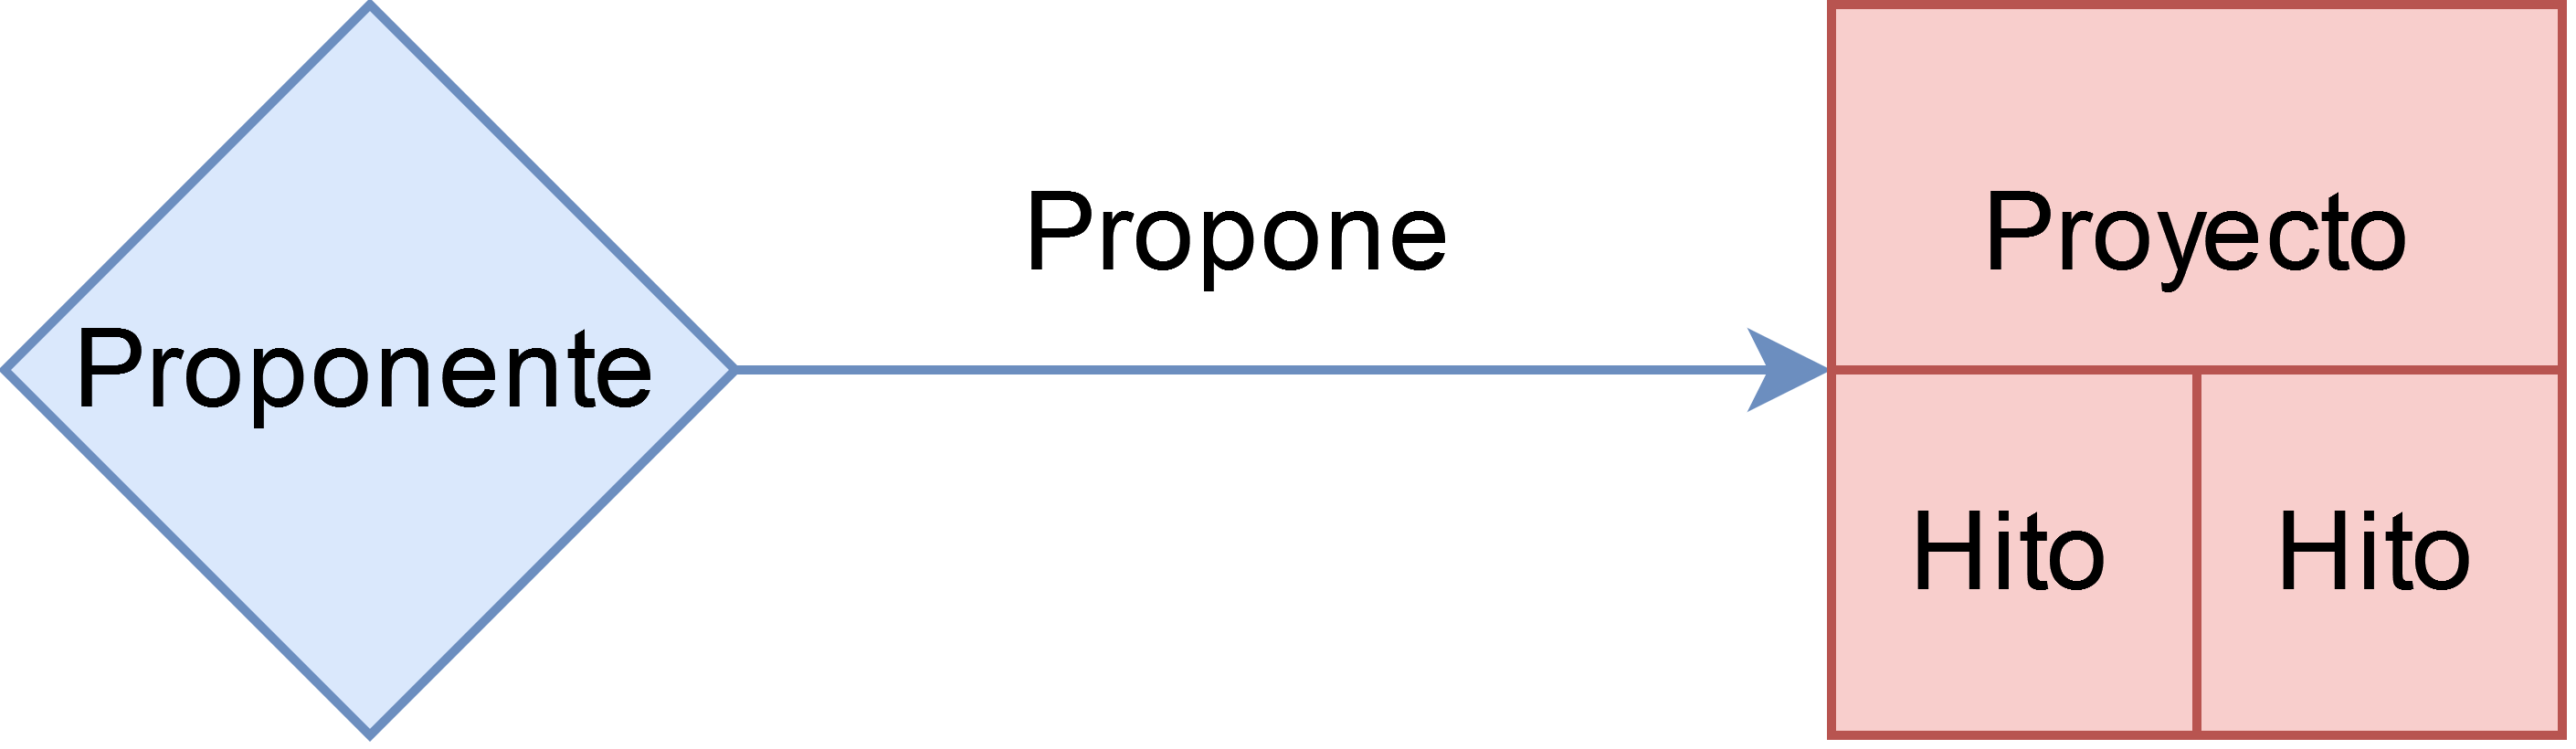
\includegraphics[width=0.45\textwidth]{img/diagramas/proponente.png}
        \caption{Diagrama de Agentes - Interacción de un proponente con un proyecto.}
        \label{fig:configApi}
\end{figure}

\subsubsection{Votantes}

Los \quotes{votantes} de este sistema es un participante activo en la toma de decisiones sobre qué proyectos se deberían financiar y cuáles no. Los votantes deciden si un proyecto debe pasar a la fase de recaudación.

\begin{figure}[H]
        \centering
        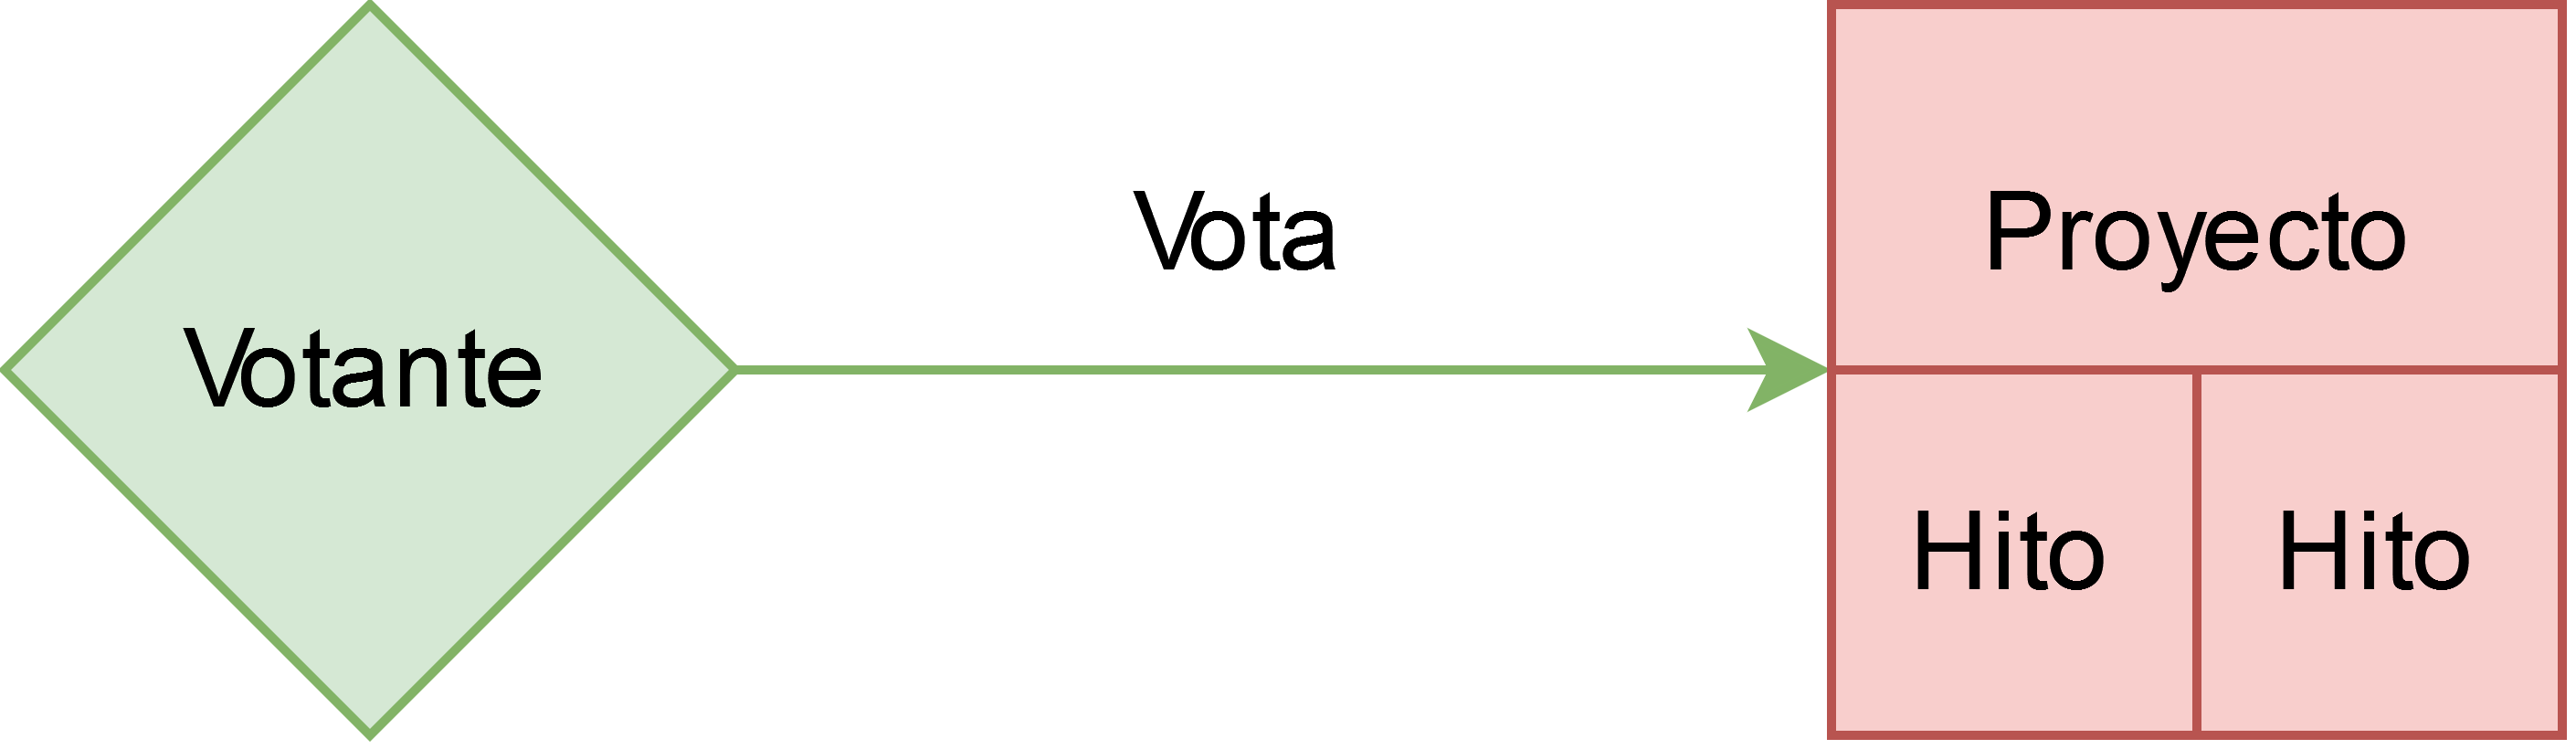
\includegraphics[width=0.45\textwidth]{img/diagramas/votante.png}
        \caption{Diagrama de Agentes - Interacción de un votante con un proyecto.}
        \label{fig:configApi}
\end{figure}


\subsubsection{Inversor}

Los \quotes{Inversores} son los usuarios que financian los proyectos que han sido aprobados por la comunidad con la garantía de que parte de su inversión está protegido en caso de que el proyecto no se lleve a cabo total o parcialmente.

\begin{figure}[H]
        \centering
        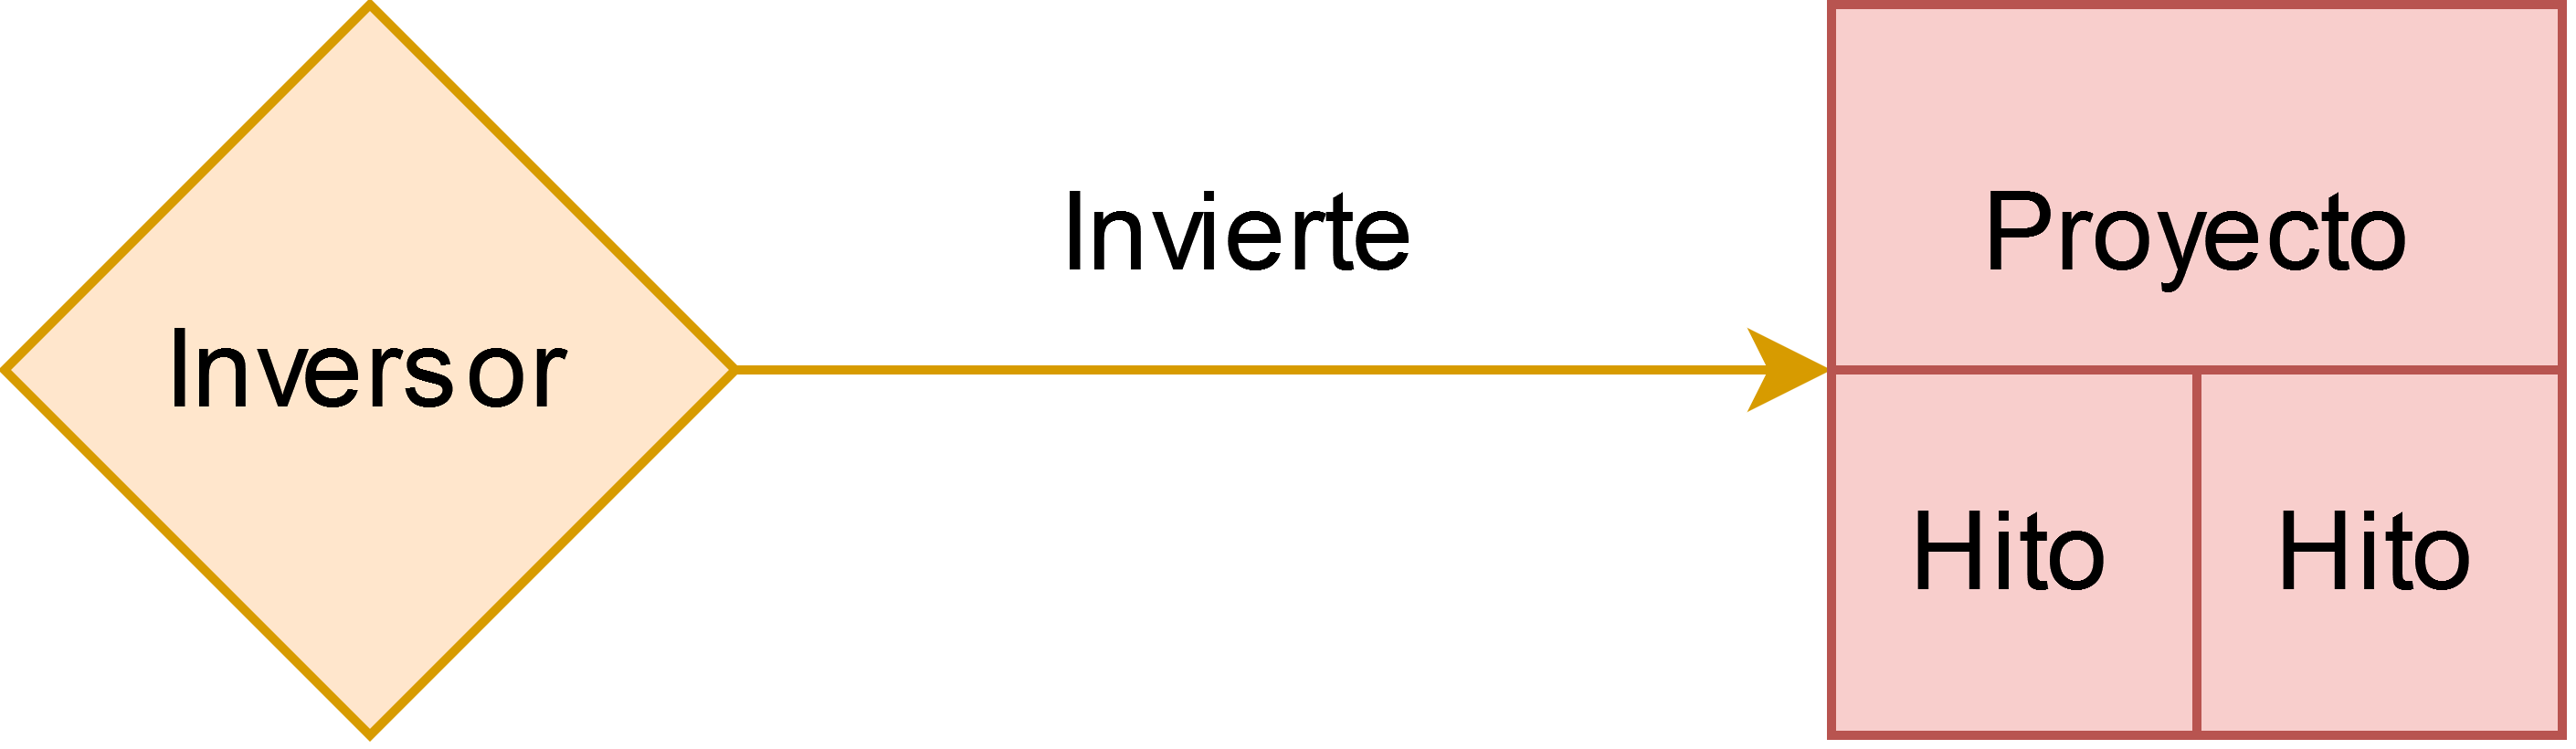
\includegraphics[width=0.45\textwidth]{img/diagramas/inversor.png}
        \caption{Diagrama de Agentes - Interacción de un inversor con un proyecto.}
        \label{fig:configApi}
\end{figure}

\bigskip

\subsubsection{Perito}

Los \quotes{Peritos} son usuarios expertos en ciertos campos relacionados con la naturaleza de los proyectos que se financian en la plataforma. Un usuario para ser perito debe poseer la acreditación necesaria de la especialización en el campo en el que dice especializarse además de una identificación personal.
Los peritos se encargan de revisar y validar que un hito se ha cumplido realmente.

\bigskip

Para validar que una acreditación es real y está en conformidad con la normativa del centro que lo ha expedido, este deberá seguir el standard \quotes{Verifiable Credentials Data Model}\cite{w3c} de W3C.

\begin{figure}[H]
        \centering
        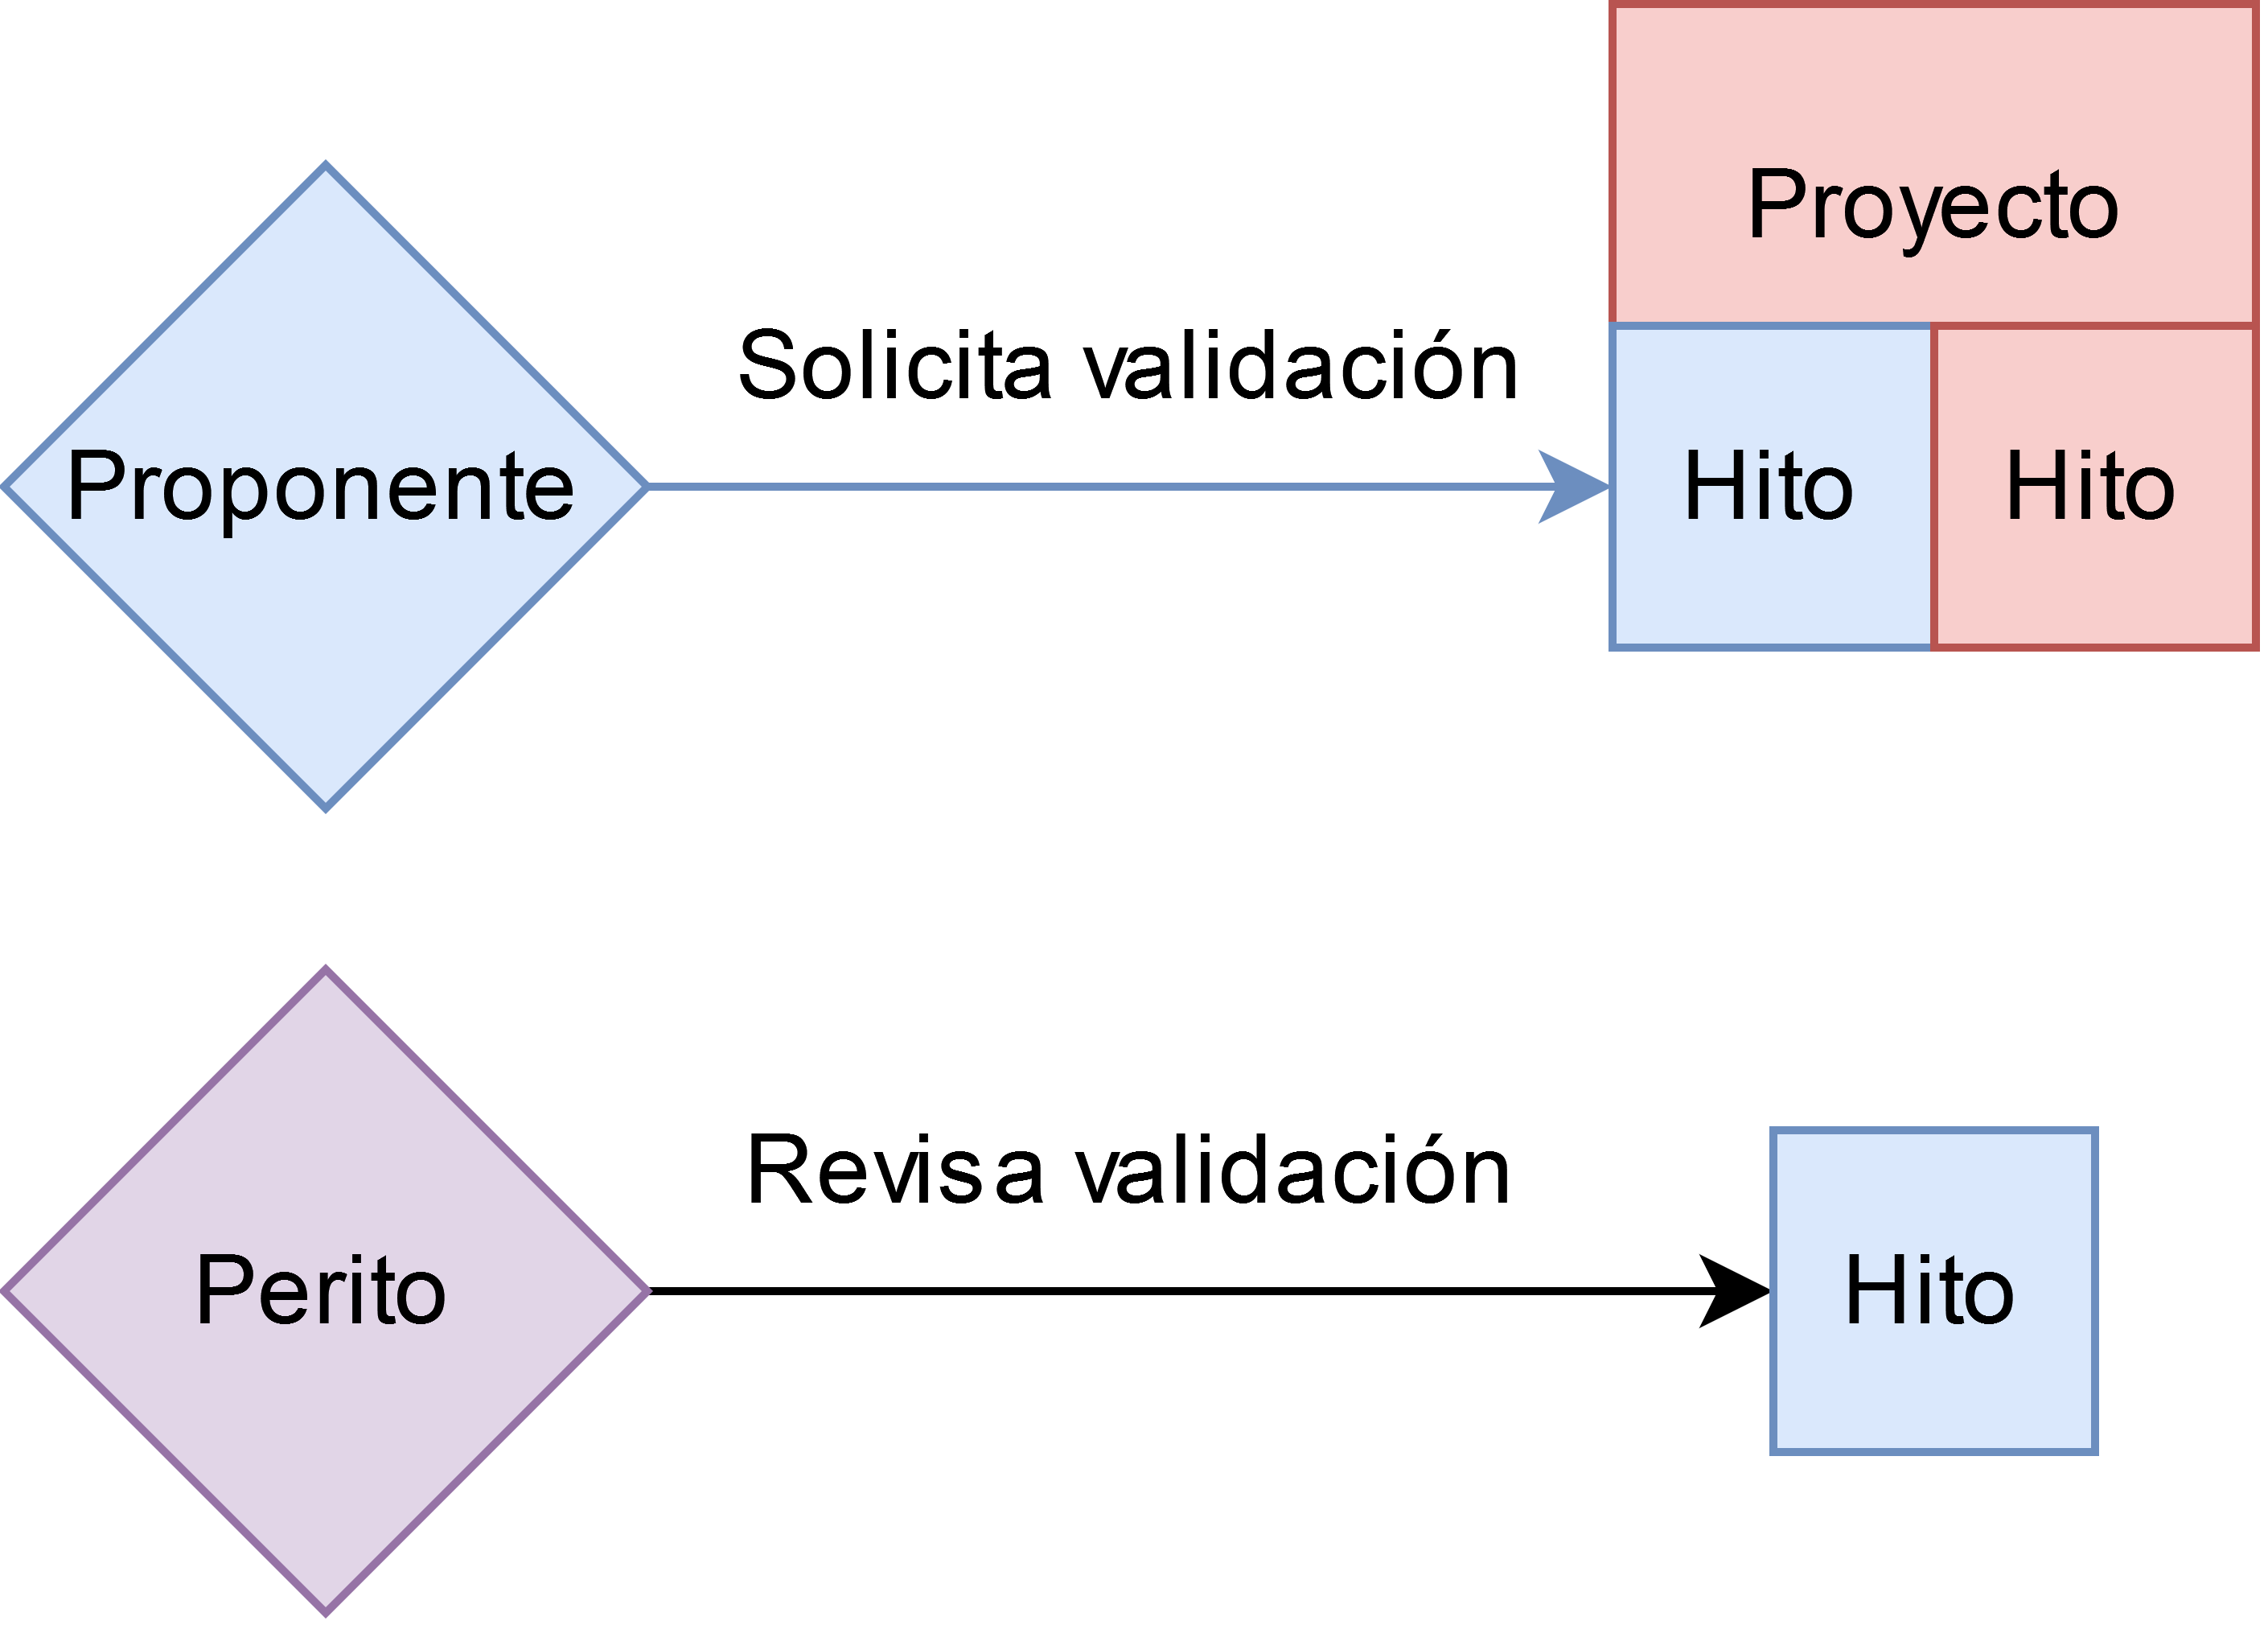
\includegraphics[width=0.45\textwidth]{img/diagramas/perito.png}
        \caption{Diagrama de Agentes - Interacción de un perito con un proyecto.}
        \label{fig:configApi}
\end{figure}

\newpage

\subsection{Interacción entre Agentes}

En el siguiente diagrama se muestra los agentes en el sistema y su proceso interactuando con un proyecto.

\begin{figure}[H]
        \centering
        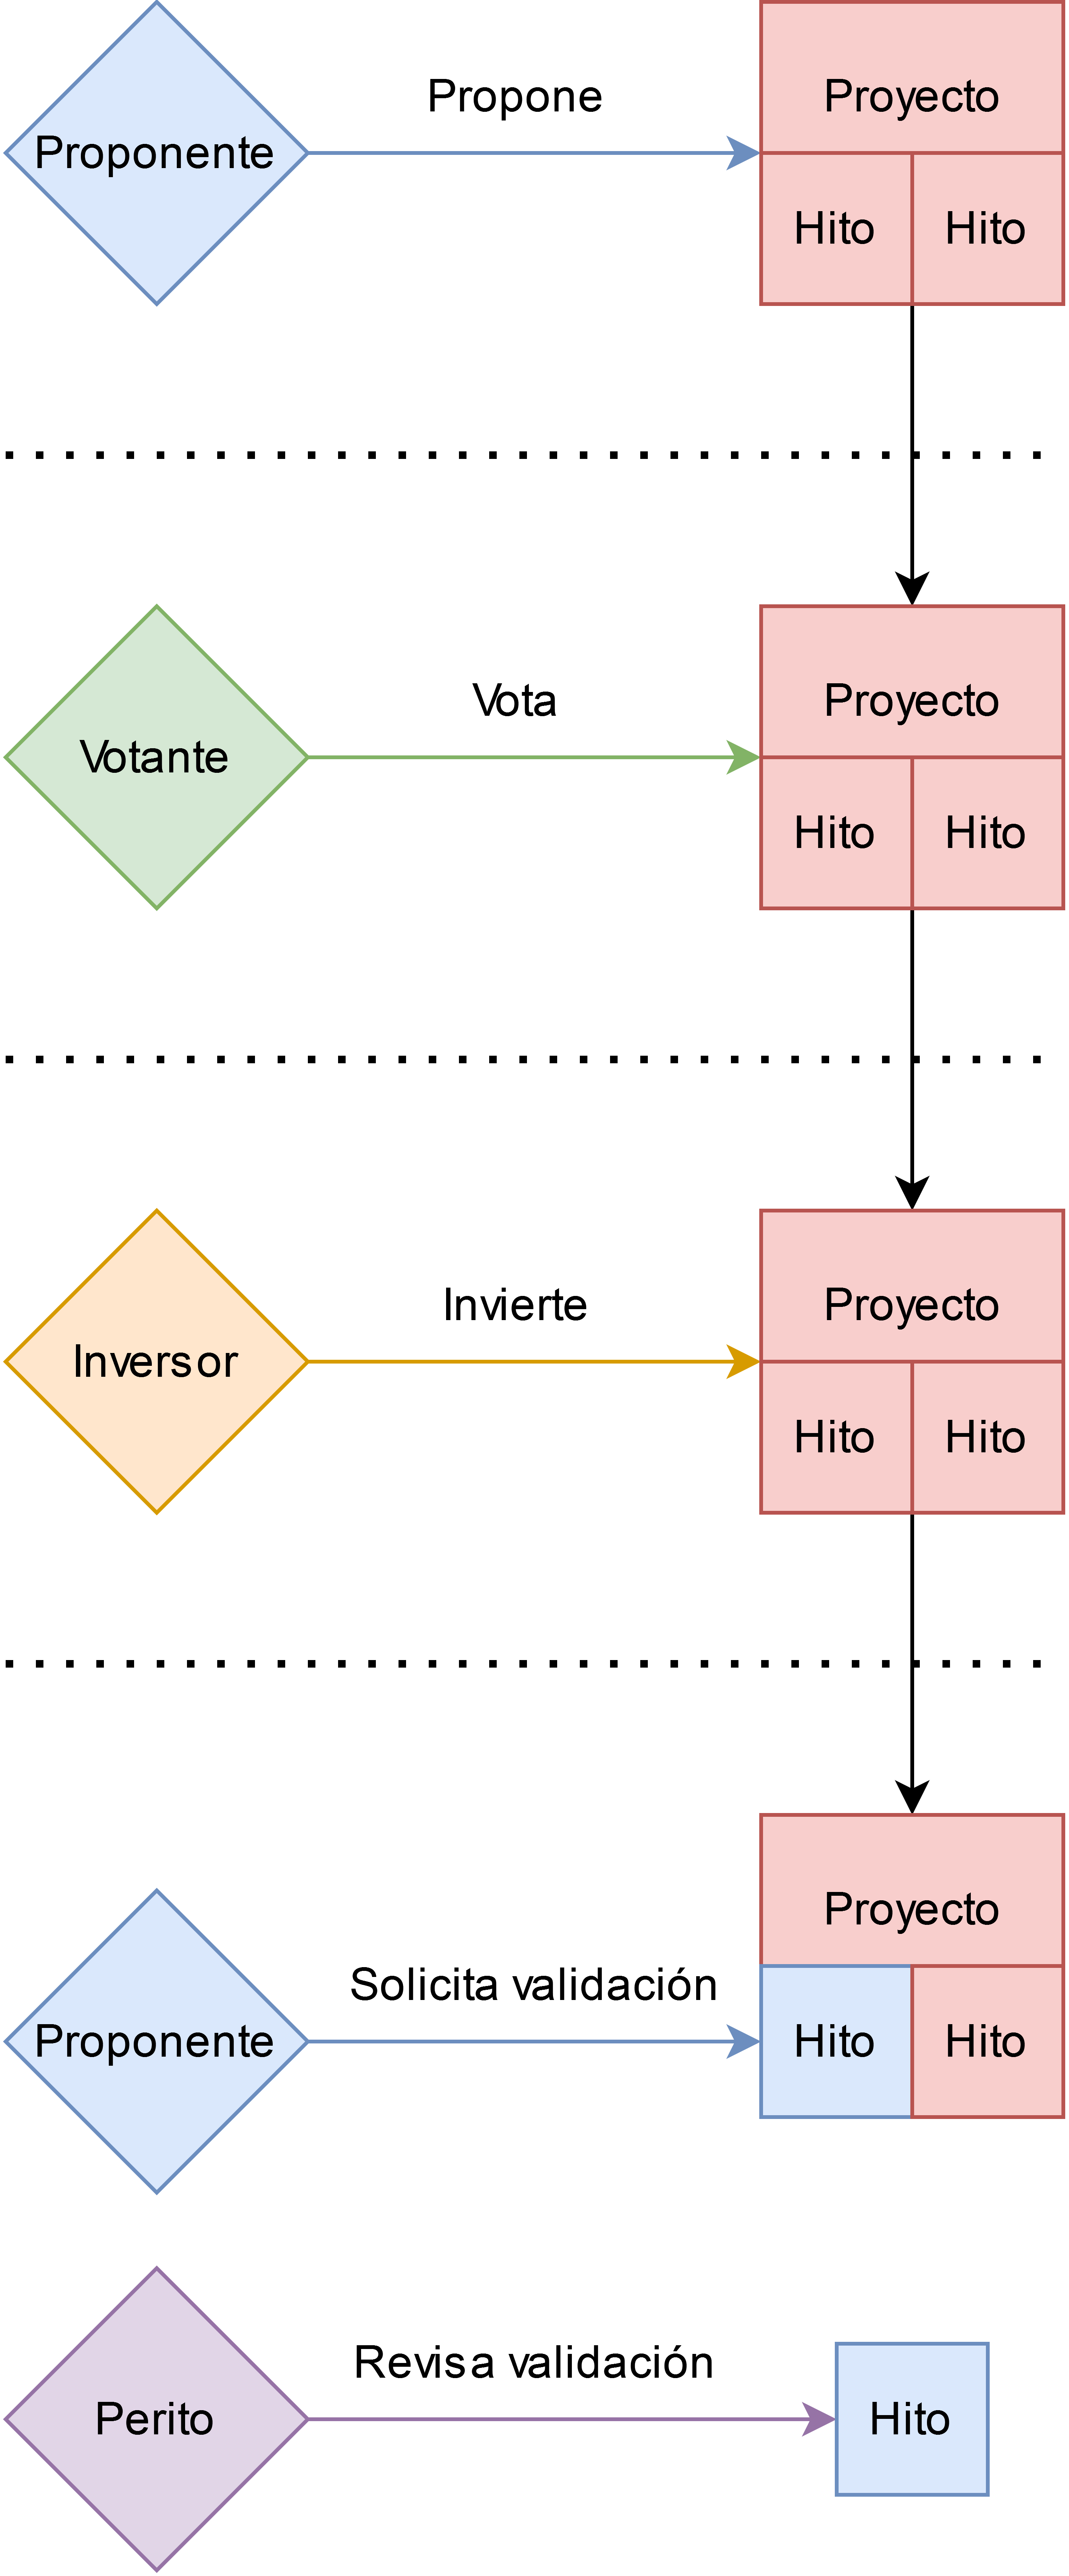
\includegraphics[width=0.45\textwidth]{img/diagramas/agentes.png}
        \caption{Diagrama de Agentes - Interacción de los agentes en el sistema a lo largo de un proyecto.}
        \label{fig:configApi}
\end{figure}

\subsection{Requerimientos}

Estas especificaciones se detallan en 3 tablas, la primera para los requerimientos funcionales y segunda para los requerimientos no funcionales además de mencionar en una tercera tabla los requerimientos que se no se implementarán en la prueba de concepto.


\subsubsection{Requerimientos Funcionales}

\begin{table}[H]
\centering
\begin{tabular}{|p{1cm}|p{4cm}|p{10cm}|}
\hline
    \textbf{ID} & \textbf{Requerimiento} & \textbf{Descripción} \\
    \hline 
    RF1 & Autenticación & Los usuarios podrán autenticarse en el sistema mediante su cartera. \\
    \hline
    RF2 & Notificación de red equivocada & Se le notificará al usuario si se ha conectado desde una red blockchain donde el contrato no está desplegado. \\
    \hline
    RF3 & Notificación de cartera no detectada & Se le notificará al usuario de que no posee ninguna cartera conectada al navegador. \\
    \hline
    RF4 & Propuesta de proyectos & Los usuarios pueden proponer nuevos proyectos. \\
    \hline 
    RF5 & Listado de proyectos & Los usuarios podrán ver todos los proyectos en la página principal de la web. \\
    \hline
    RF6 & Añadir comentarios & Los usuarios pueden realizar comentarios sobre un proyecto en la página del proyecto. \\
    \hline
    RF7 & Leer comentarios & Los usuarios pueden leer los comentarios sobre un proyecto en la página del proyecto. \\
    \hline
    RF8 & Votación de proyectos & Los usuarios pueden votar para aprobar o rechazar proyectos propuestos. \\
    \hline
    RF9 & Aprobación del proyecto & Un proyecto es aprobado si alcanza al menos el 85 \% de votos positivos en un plazo de 30 días desde su propuesta. De lo contrario, se rechaza. \\
    \hline
    RF10 & Financiación del proyecto & Los usuarios pueden invertir en proyectos aprobados. \\
    \hline
    RF11 & Solicitud de Validación de hitos & El proponente solicitará a la comunidad validar el siguiente hito. \\
    \hline
    RF12 & Validación de hitos & Los peritos validarán una solicitud, así confirmando o denegando si se ha alcanzado el objetivo del hito. \\
    \hline
    RF13 & Liberación de fondos & Permite al proponente obtener los fondos asignados de un hito validado. \\
    \hline
    RF14 & Subsanación de hitos & Si la validación de un hito acaba siendo denegada por la comunidad, el proponente tiene 10 días para abordar los problemas propuestos, y solicitar nuevamente la validación del hito. \\
    \hline
    RF15 & Cancelación de proyecto & Un proyecto se cancela automáticamente si muestra signos de estancamiento en un hito, o no el proponente deja de comunicarse. \\
    \hline
    RF16 & Procesado de archivos & El sistema tendrá una funcionalidad en el frontend capaz de subir archivo a IPFS para su publicación en dicha blockchain. \\
    \hline
    
\end{tabular}
\caption{Análisis y Diseño - Requerimientos funcionales del sistema.}
\label{tab:requisitos_funcionales}
\end{table}

\newpage

\subsubsection{Requerimientos no Funcionales}

\begin{table}[H]
\centering
\begin{tabular}{|p{1cm}|p{3cm}|p{10cm}|}
    \hline
    \textbf{ID} & \textbf{Requerimiento} & \textbf{Descripción} \\
    \hline
    RNF1 & Seguridad & El sistema debe garantizar la seguridad de los fondos y los datos, evitando ataques y accesos no autorizados. \\
    \hline
    RNF2 & Escalabilidad & El sistema debe ser capaz de manejar un creciente número de usuarios y proyectos sin degradar el rendimiento. \\
    \hline
    RNF3 & Interoperabilidad & El sistema debe ser compatible con diversas plataformas y tecnologías blockchain, permitiendo la interacción con otros sistemas y servicios. \\
    \hline
    RNF4 & Eficiencia & El sistema debe optimizar el uso de recursos y reducir costos operativos, incluyendo tarifas de transacción en la blockchain. \\
    \hline
    RNF5 & Usabilidad & La interfaz de usuario debe ser intuitiva y fácil de usar para permitir a usuarios de diversos niveles de experiencia interactuar con el sistema. \\
    \hline
    RNF6 & Transparencia & El sistema debe proporcionar a los usuarios información clara y accesible sobre el proceso de votación, financiación y validación de hitos. \\
    \hline
    RNF7 & Confiabilidad & El sistema debe ser robusto y resistente a fallos, asegurando la disponibilidad continua del servicio. \\
    \hline
    RNF8 & Mantenibilidad & El diseño del sistema debe facilitar la actualización, mejora y corrección de errores en el futuro. \\
    \hline
    RNF9 & Legalidad & El sistema debe cumplir con las regulaciones y leyes aplicables en las jurisdicciones en las que opera. \\
    \hline
    RNF10 & Privacidad & El sistema debe proteger la privacidad de los usuarios, almacenando y gestionando sus datos de manera segura y de acuerdo con las leyes de protección de datos. \\
    \hline
    RNF11 & Trazabilidad y control & El sistema garantiza la trazabilidad y el control de los fondos y activos de la plataforma. \\
    \hline
    RNF12 & Inmutabilidad & Los datos del proyecto, una vez aprobados, no pueden ser eliminados ni modificados. \\
    \hline
    RNF13 & Sistema basado en Roles & Los agentes se distribuirán usando el estandard de roles access-control de OpenZeppelin. \\
    \hline
\end{tabular}
\caption{Análisis y Diseño - Requerimientos no funcionales del sistema.}
\label{tab:non_functional_requirements}
\end{table}

\newpage

\subsubsection{Requisitos excluidos}

En el capitulo número 7 de este documento se presenta la evaluación de la prueba de concepto correspondiente a la propuesta desarrollada. Dado que se trata únicamente de una prueba del concepto el sistema implementado que se llevara a cabo se considera como una muestra de la propuesta de solución, ya que el tiempo correspondiente al trabajo ( 12 ECTS - 300 Horas ) no es el suficiente para realizar la implementación completa de la solución propuesta.

\bigskip

También teniendo en cuenta que esta solución es una prueba de concepto, se ha considerado no indagar en profundidad en los aspectos legales del tratamiento de datos con respecto a los agentes.

\bigskip

En consecuencia, en este apartado se enumeran los requerimientos que no se han llevado a cabo debido a la limitación de tiempo y a que sobrepasan de los limites demandados para este trabajo:

\begin{table}[H]
\centering
\begin{tabular}{|p{5cm}|}
\hline
    \textbf{Requerimientos.} \\
    \hline
    RF11 \\
    \hline
    RF12 \\
    \hline
    RF14 \\
    \hline
    RF16 \\
    \hline
    \hline
    RNF9 \\
    \hline
    RNF13 \\
    \hline
\end{tabular}
\caption{Análisis y Diseño - Requerimientos no implementados en la prueba de concepto.}
\label{tab:requisitos_no_funcionales}
\end{table}

\subsection{Gobernanza}

La gobernanza del sistema propuesto se basa en un enfoque descentralizado, aprovechando la tecnología blockchain para gestionar de manera eficiente y transparente la financiación de proyectos.

\bigskip

La plataforma opera mediante un mecanismo de gestión autónomo, lo que elimina la necesidad de un administrador central y reduce el riesgo de malversación de fondos.

\bigskip

Esto se debe gracias a que el protocolo Ethereum permite la ejecución de smart contracts, código personalizado que una vez desplegado es inalterable.

\bigskip

Esto nos permite definir sistemas que pueden ser autogobernables con una gobernanza regida por el código (code-as-law), sin necesidad de un actor administrador.

\newpage

\subsection{Diseños}

A continuación se muestran los diseños del sistema, tales como los diagramas de flujo del sistema y los mockups de la interfaz.

\subsubsection{Diagrama de Flujo}

El diagrama a continuación representa de forma generalizada el flujo del sistema.

\paragraph{Proceso de contribución en un proyecto}
\begin{figure}[H]
        \centering
        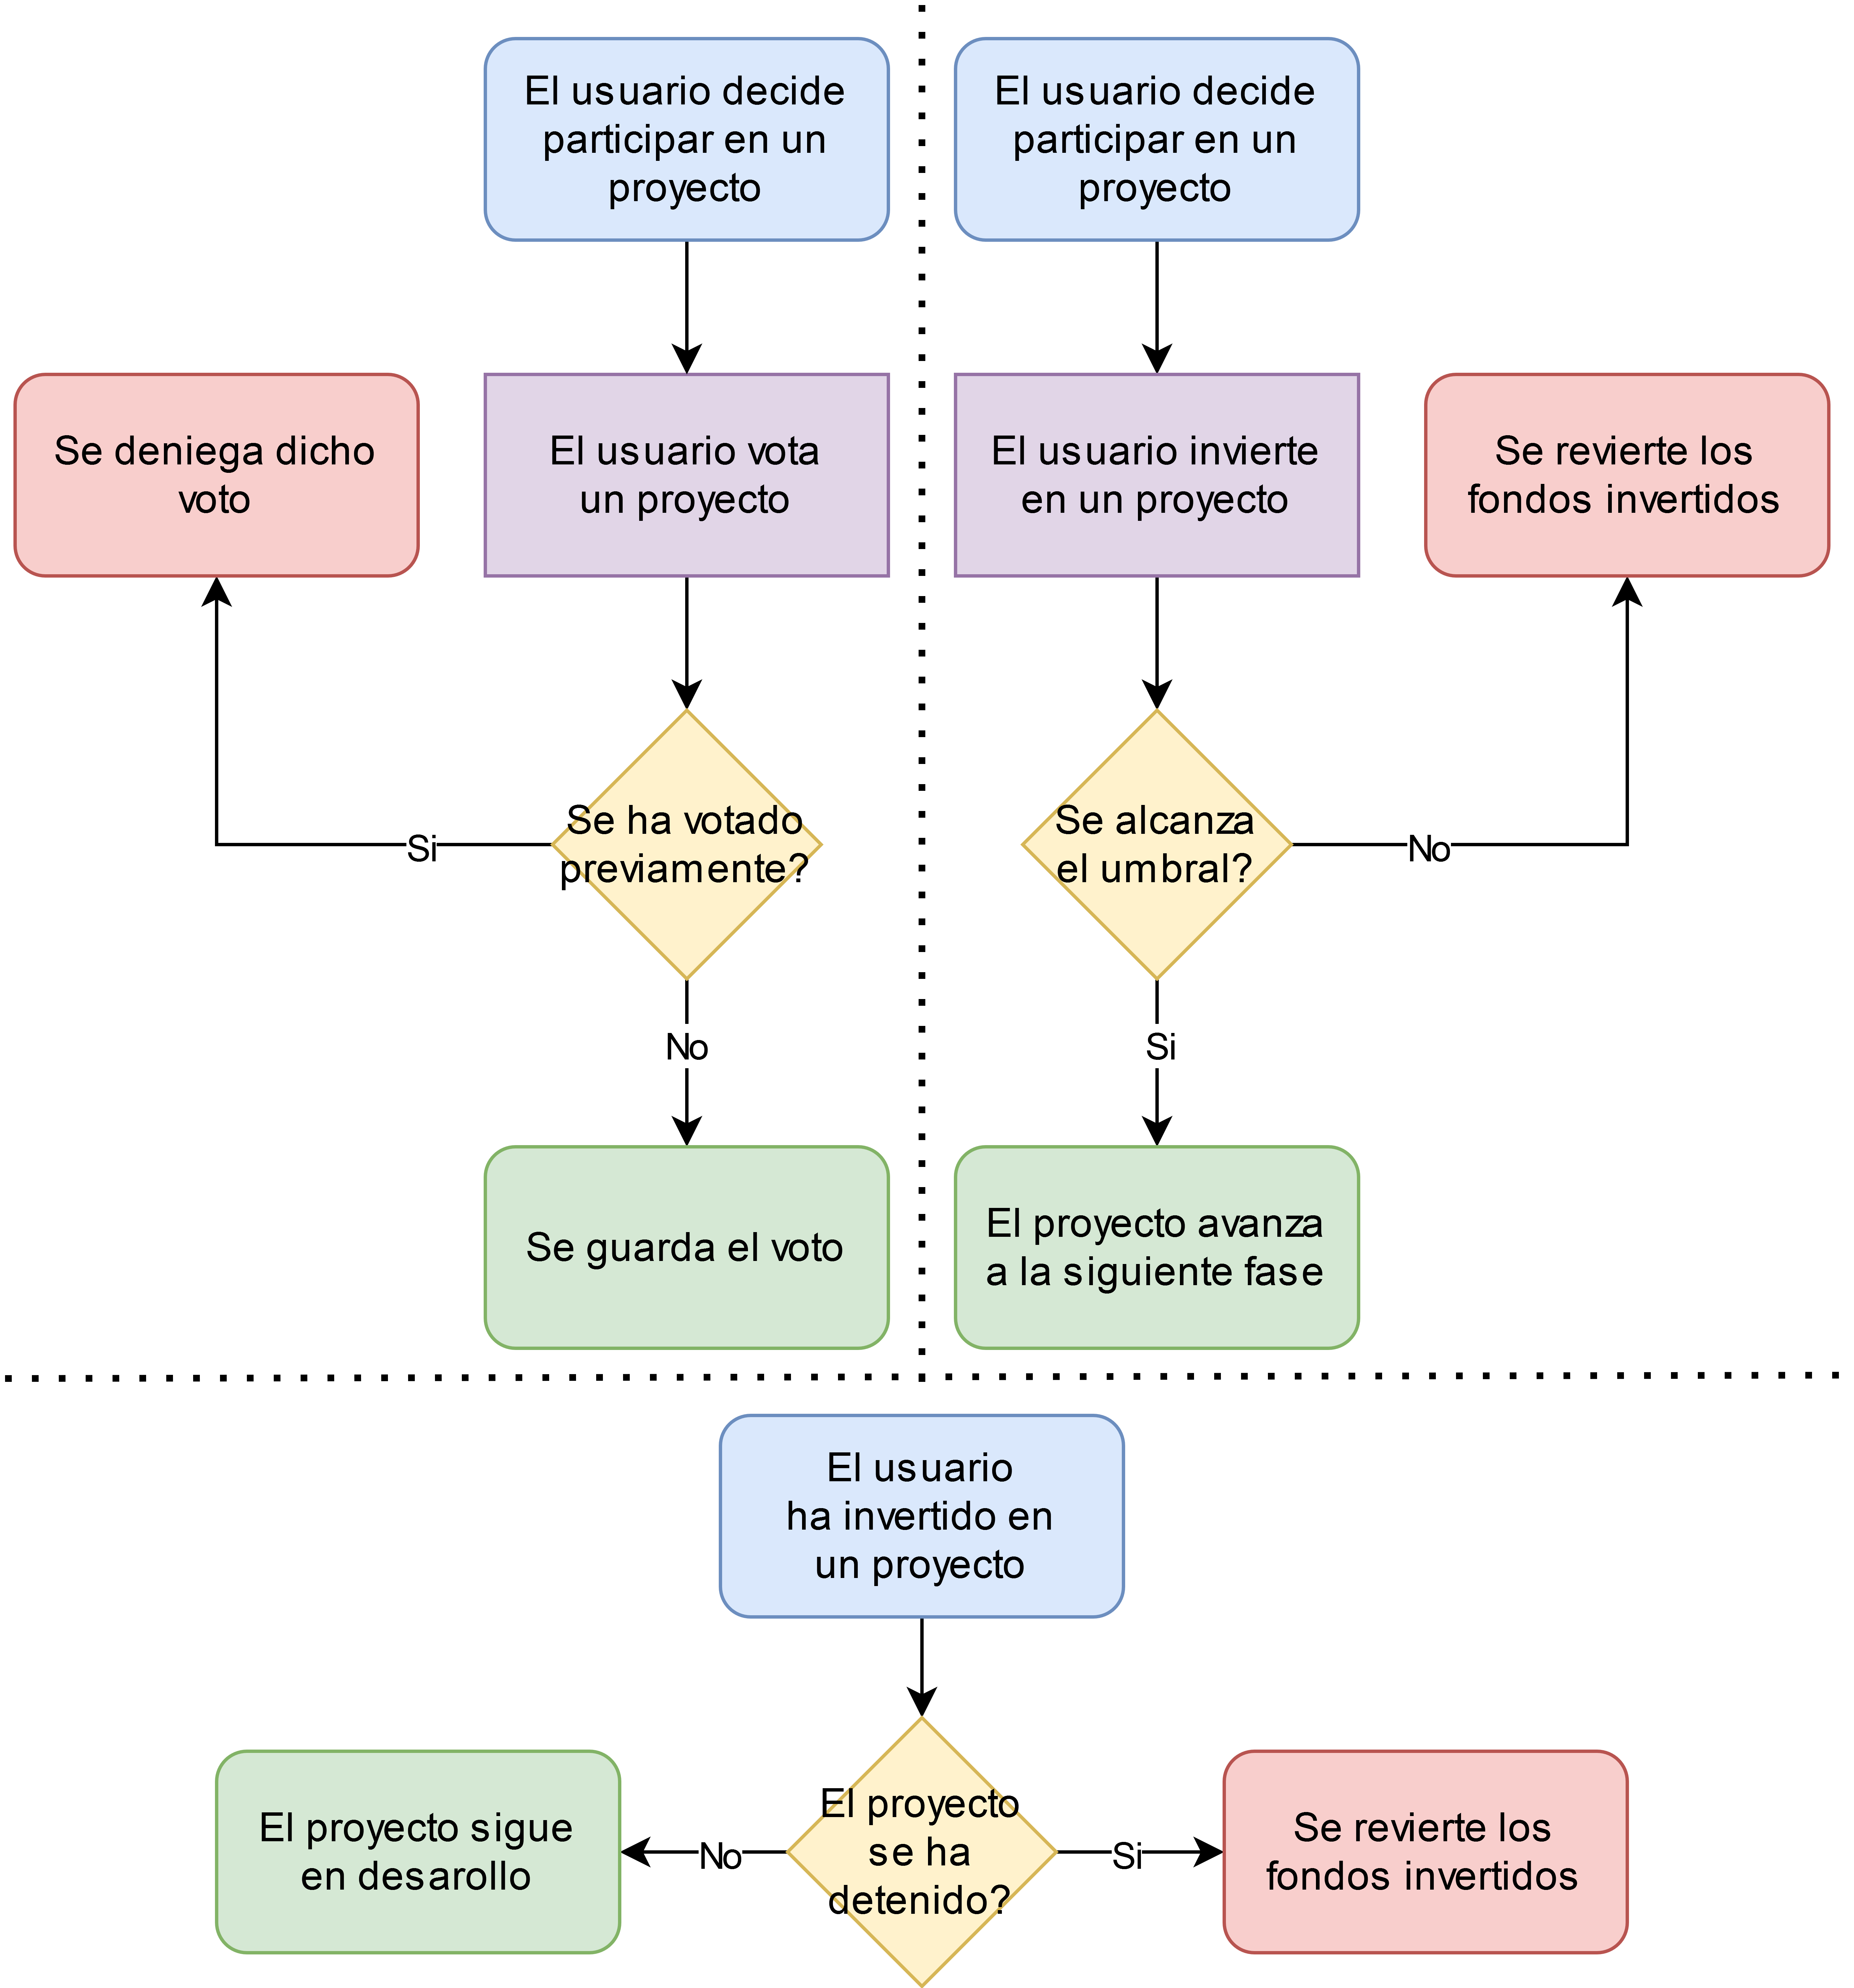
\includegraphics[width=0.8\textwidth]{img/diagramas/diagrama_flujo_votante.png}
        \caption{Diagrama de Flujo - Proceso de contribución con un proyecto.}
        \label{fig:configApi}
\end{figure}



\newpage

\paragraph{Proceso de propuesta de un nuevo proyecto}
\begin{figure}[H]
        \centering
        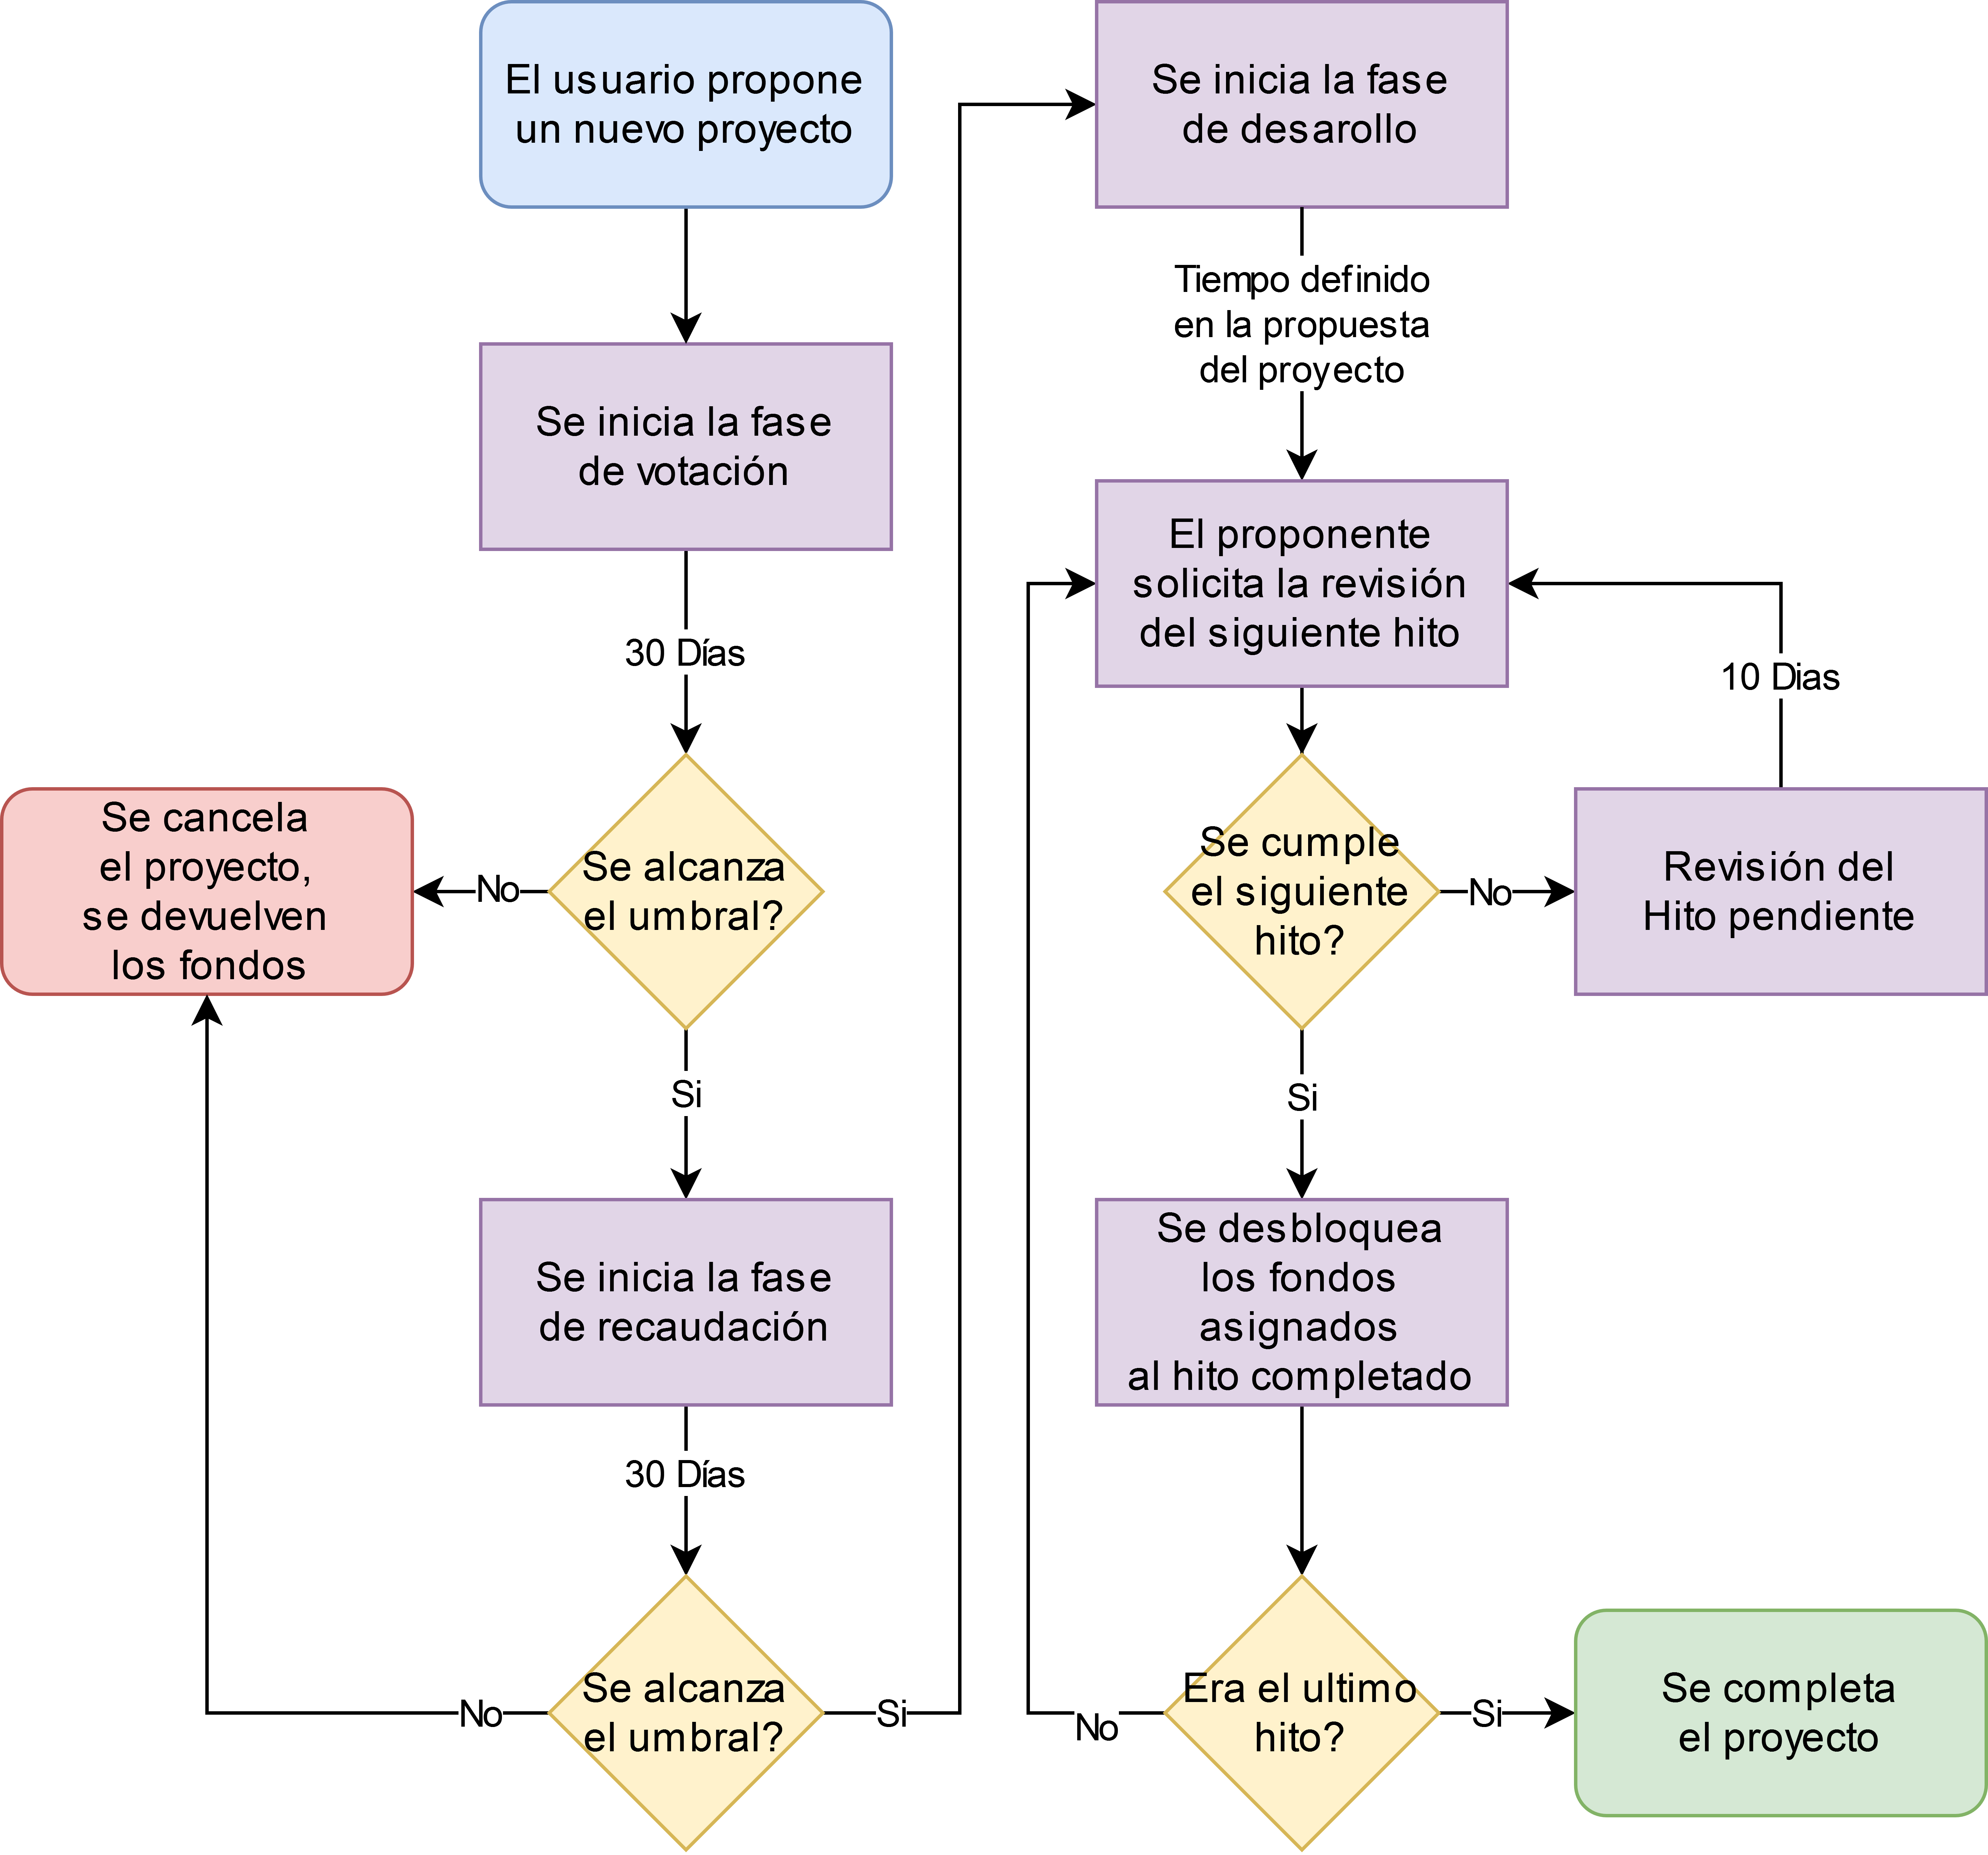
\includegraphics[width=0.8\textwidth]{img/diagramas/diagrama_flujo_proponente.png}
        \caption{Diagrama de Flujo - Proceso de propuesta de proyecto.}
        \label{fig:configApi}
\end{figure}

\newpage

\subsubsection{Mockups}

A continuación se mostrarán los mockups del diseño del de la interfaz (front-end) a desarrollar para la prueba de concepto.

\bigskip

Para abarcar los requerimientos funcionales, se ha desarrollado una interfaz donde cada pantalla provee la interacción necesaria para cumplir con los requerimientos a implementar en la prueba de concepto.

\paragraph{Pantalla de Registro}
\begin{figure}[H]
        \centering
        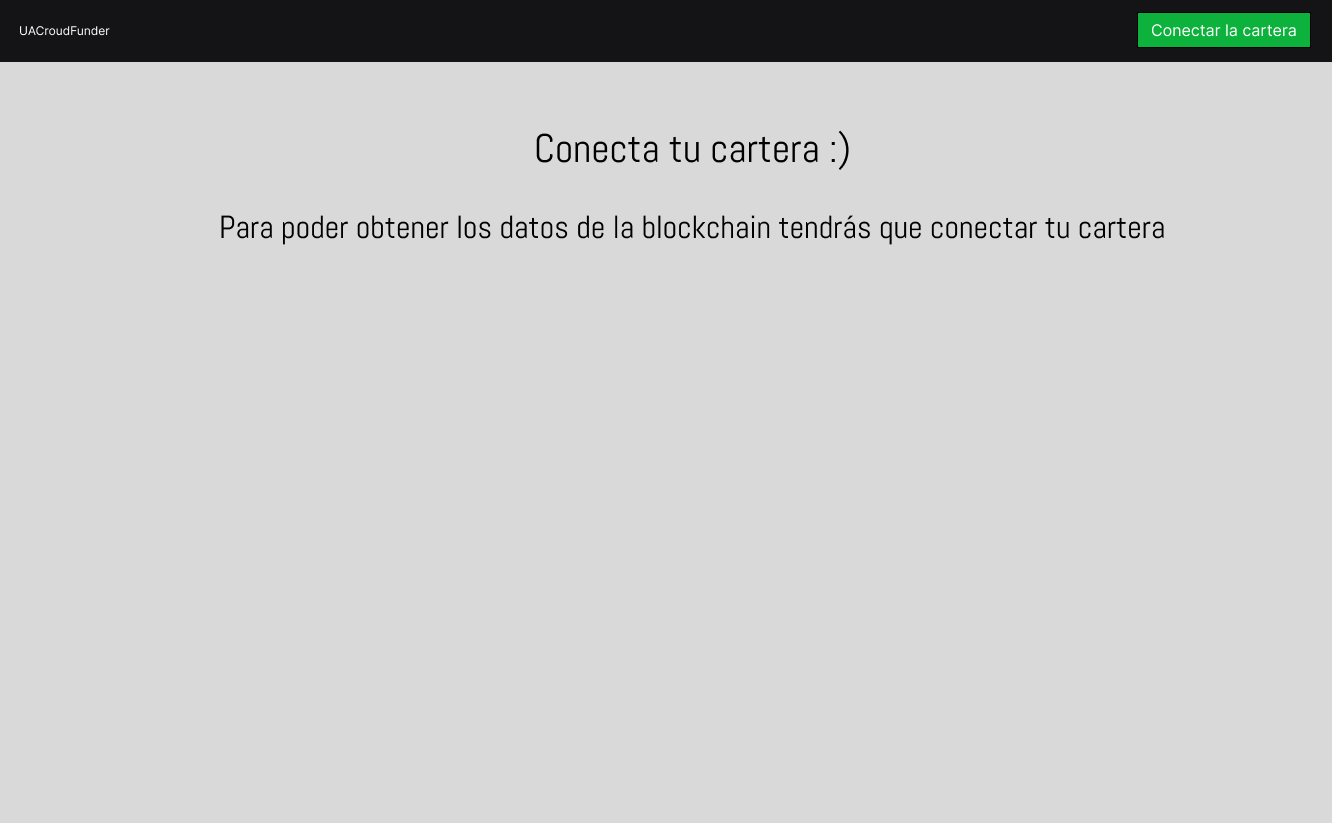
\includegraphics[width=1\textwidth]{img/mockups/pantalla_registro.png}
        \caption{Mockup - Pantalla de Registro.}
        \label{fig:configApi}
\end{figure}

En esta pantalla se mostrará un mensaje de bienvenida, y un botón con la funcionalidad para conectar la cartera al front-end.

\bigskip

\textbf{Requerimientos: }
\begin{itemize}
    \item RF1
\end{itemize}


\paragraph{Pantalla de notificación de red equivocada}
\begin{figure}[H]
        \centering
        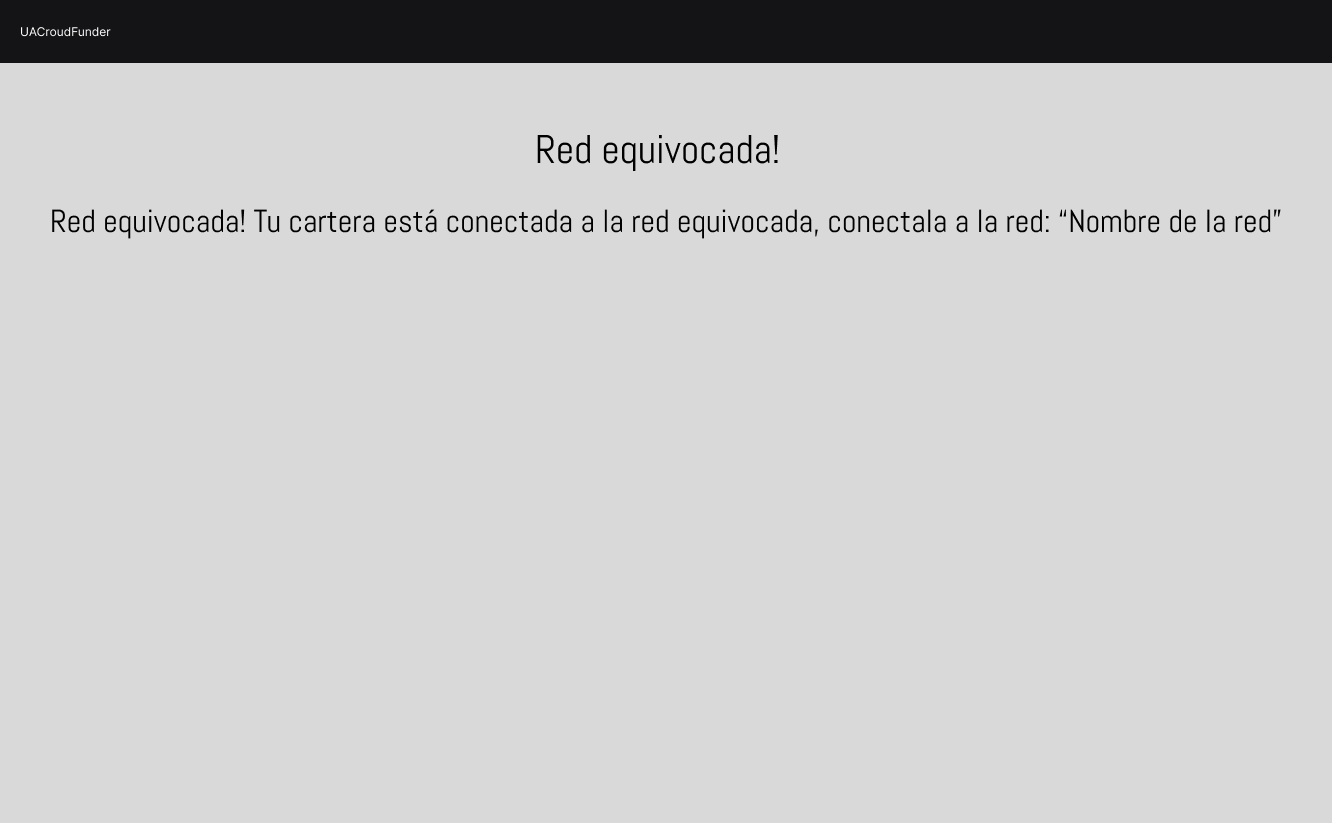
\includegraphics[width=1\textwidth]{img/mockups/red_equivocada.png}
        \caption{Mockup - Notificación de red equivocada.}
        \label{fig:configApi}
\end{figure}

En caso de que el usuario esté conectado a una red diferente a donde está desplegado el contrato, se mostrará un mensaje de advertencia y la red a la que se debe de conectar.

\bigskip

\textbf{Requerimientos: }
\begin{itemize}
    \item RF2
\end{itemize}

\paragraph{Pantalla de notificación de cartera inexistente}
\begin{figure}[H]
        \centering
        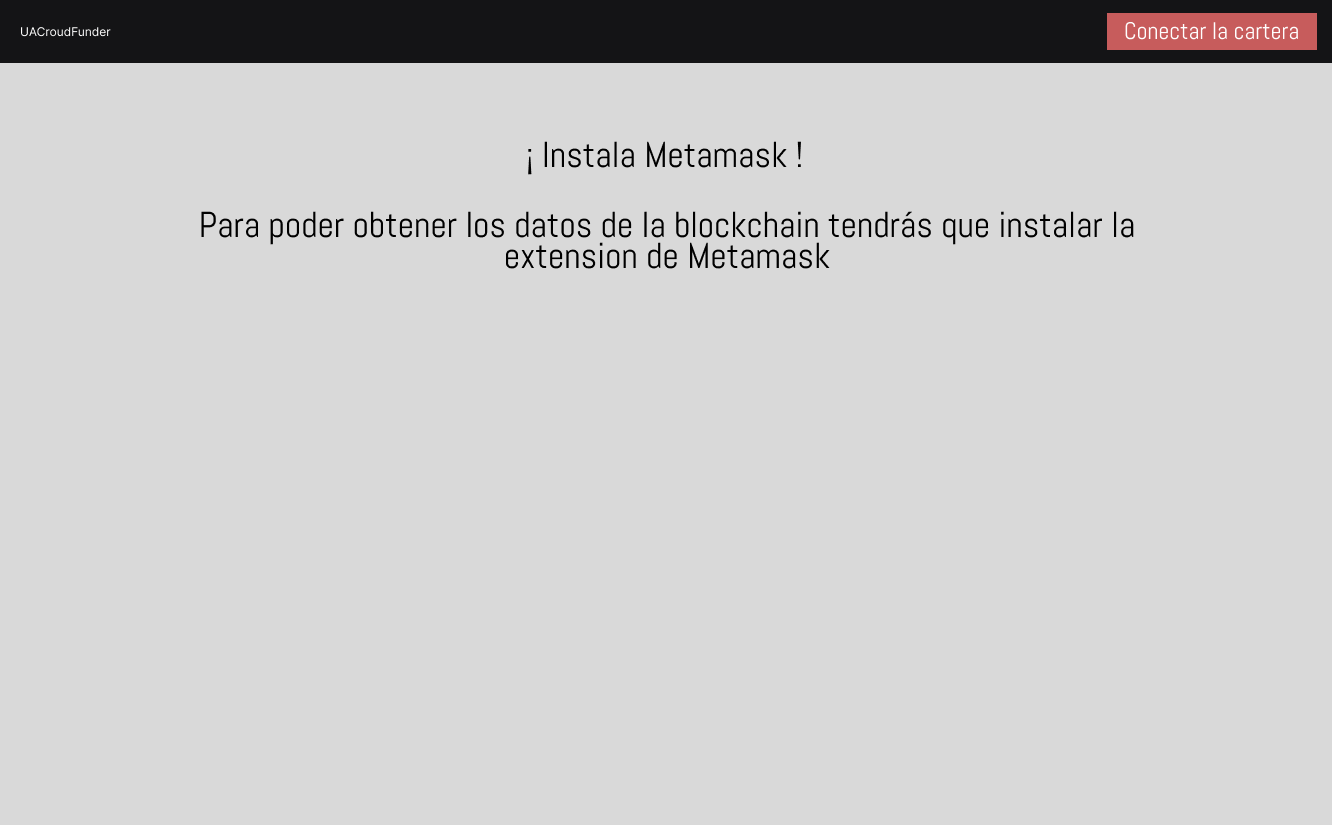
\includegraphics[width=1\textwidth]{img/mockups/cartera_inexistente_mockup.png}
        \caption{Mockup - Notificación de que la cartera no se ha detectado.}
        \label{fig:configApi}
\end{figure}

En caso de que el usuario se intente conectar pero no tenga ninguna cartera instalada en el navegador, se le notificará de la situación mediante un mensaje.

\bigskip

\textbf{Requerimientos: }
\begin{itemize}
    \item RF3
\end{itemize}

\paragraph{Pantalla de la lista de Proyectos}
\begin{figure}[H]
        \centering
        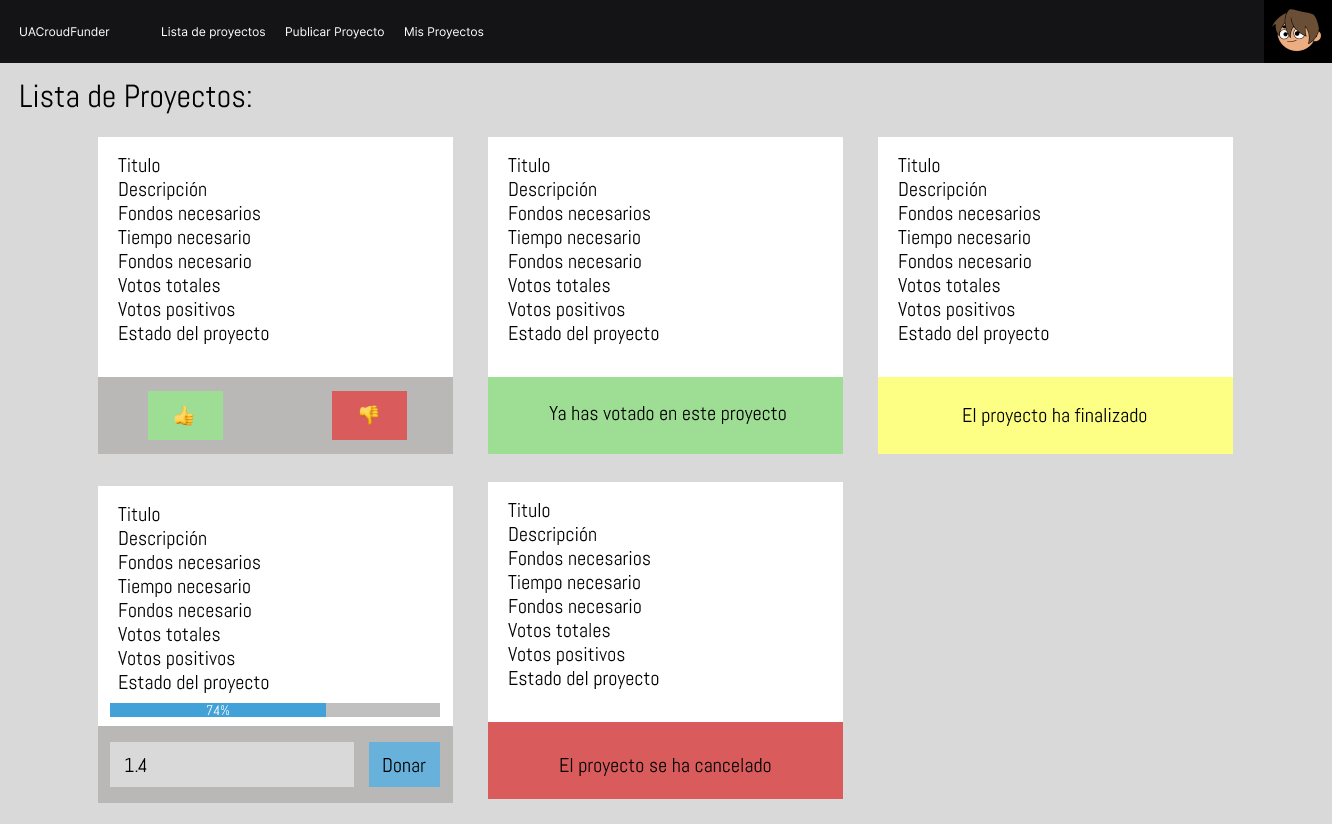
\includegraphics[width=1\textwidth]{img/mockups/lista_proyectos.png}
        \caption{Mockup - Lista de Proyectos.}
        \label{fig:configApi}
\end{figure}

En la siguiente pantalla se mostará una lista de los proyectos en forma de cards, donde se describirá sus detalles, además de poder votar y donar directamente.

\bigskip

Esta misma pantalla también servirá para filtrar por los proyectos propuestos por el propio usuario

\bigskip

\textbf{Requerimientos: }
\begin{itemize}
    \item RF5
    \item RF8
    \item RF10
\end{itemize}

\paragraph{Pantalla del formulario para proponer un proyecto}
\begin{figure}[H]
        \centering
        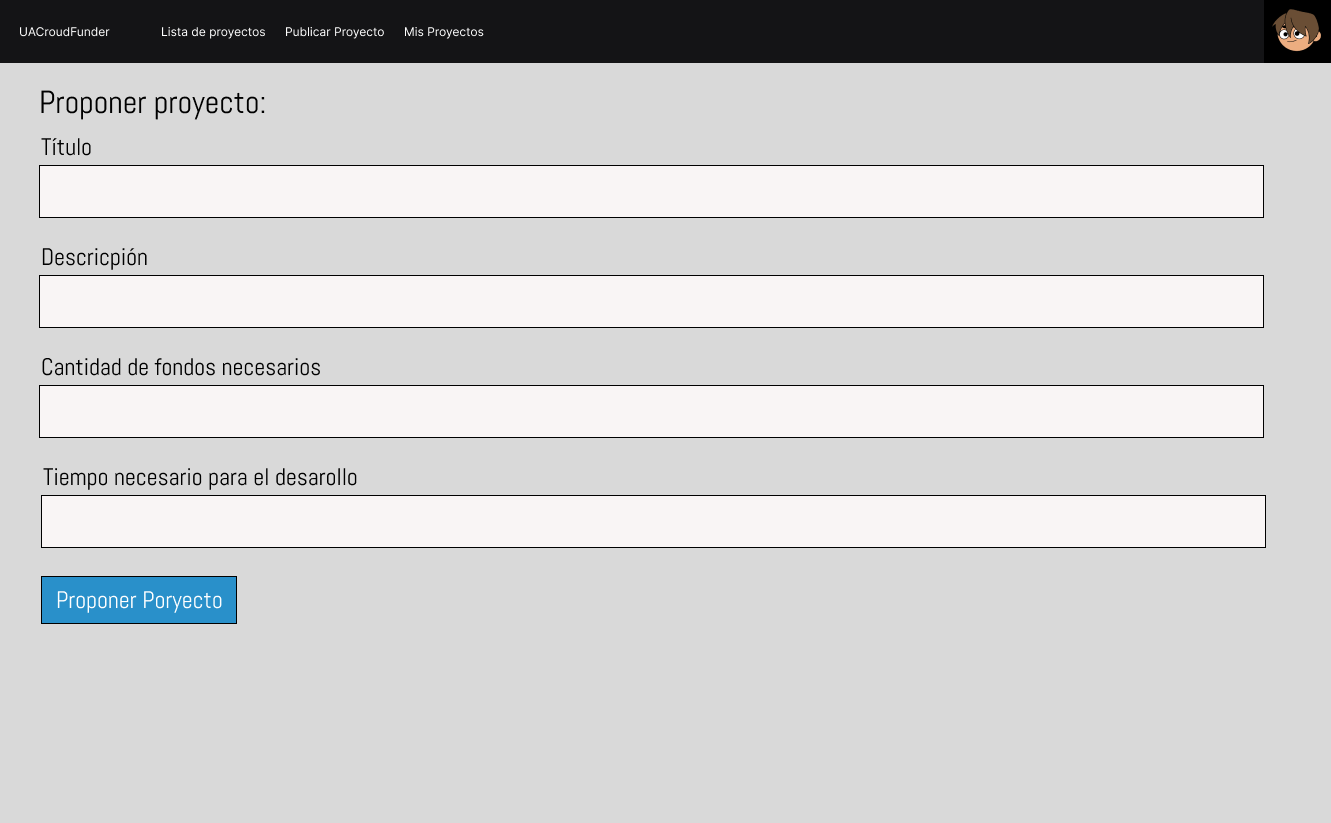
\includegraphics[width=1\textwidth]{img/mockups/proponer_proyecto.png}
        \caption{Mockup - Formulario para proponer un proyecto.}
        \label{fig:configApi}
\end{figure}

En esta pantalla se le permitirá al usuario proponer un nuevo proyecto, rellenando los datos necesarios.

\bigskip

\textbf{Requerimientos: }
\begin{itemize}
    \item RF4
\end{itemize}

\paragraph{Pantalla de detalles de un proyecto}
\begin{figure}[H]
        \centering
        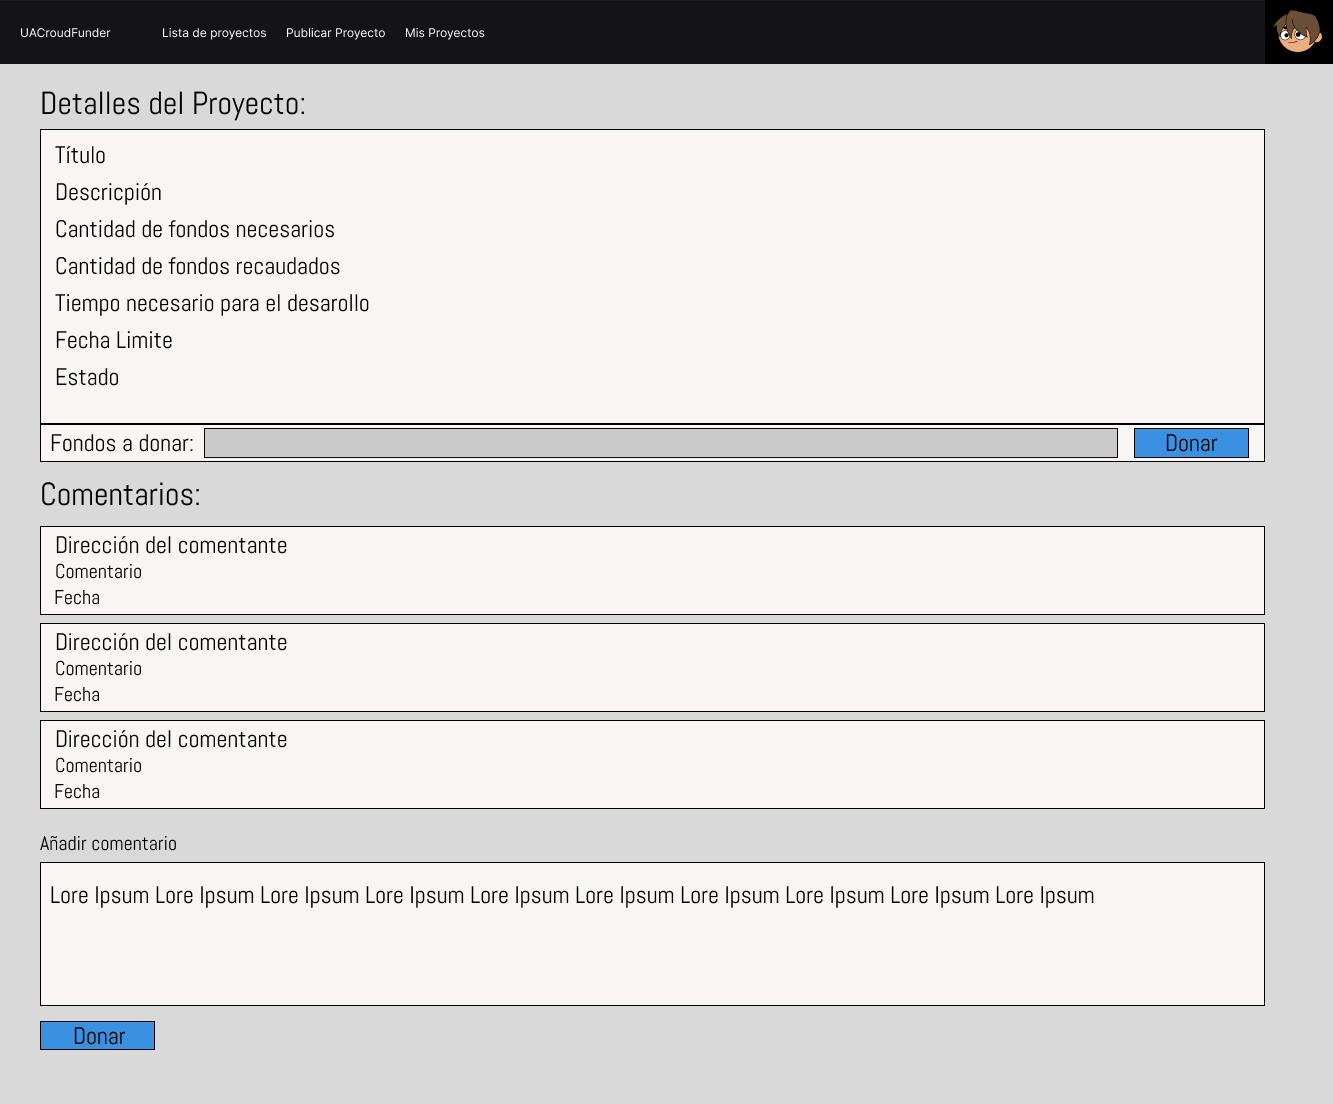
\includegraphics[width=1\textwidth]{img/mockups/detalles_proyecto.png}
        \caption{Mockup - Detalles de un proyecto.}
        \label{fig:configApi}
\end{figure}

Y en esta pantalla se mostrará en detalle los datos de un proyecto, además de las funcionalidades de votar, donar, leer y comentar sobre sobre el proyecto.

\bigskip

\textbf{Requerimientos: }
\begin{itemize}
    \item RF6
    \item RF7
    \item RF8
    \item RF10
\end{itemize}

\newpage

\subsubsection{Modelo del smart contract}

Para el desarrollo de este sistema, necesitaremos varias estructuras para gestionar los datos en el smart contract.

\bigskip

A continuación se muestra un esquema con las estructuras de datos de la solución propuesta:

\begin{figure}[H]
        \centering
        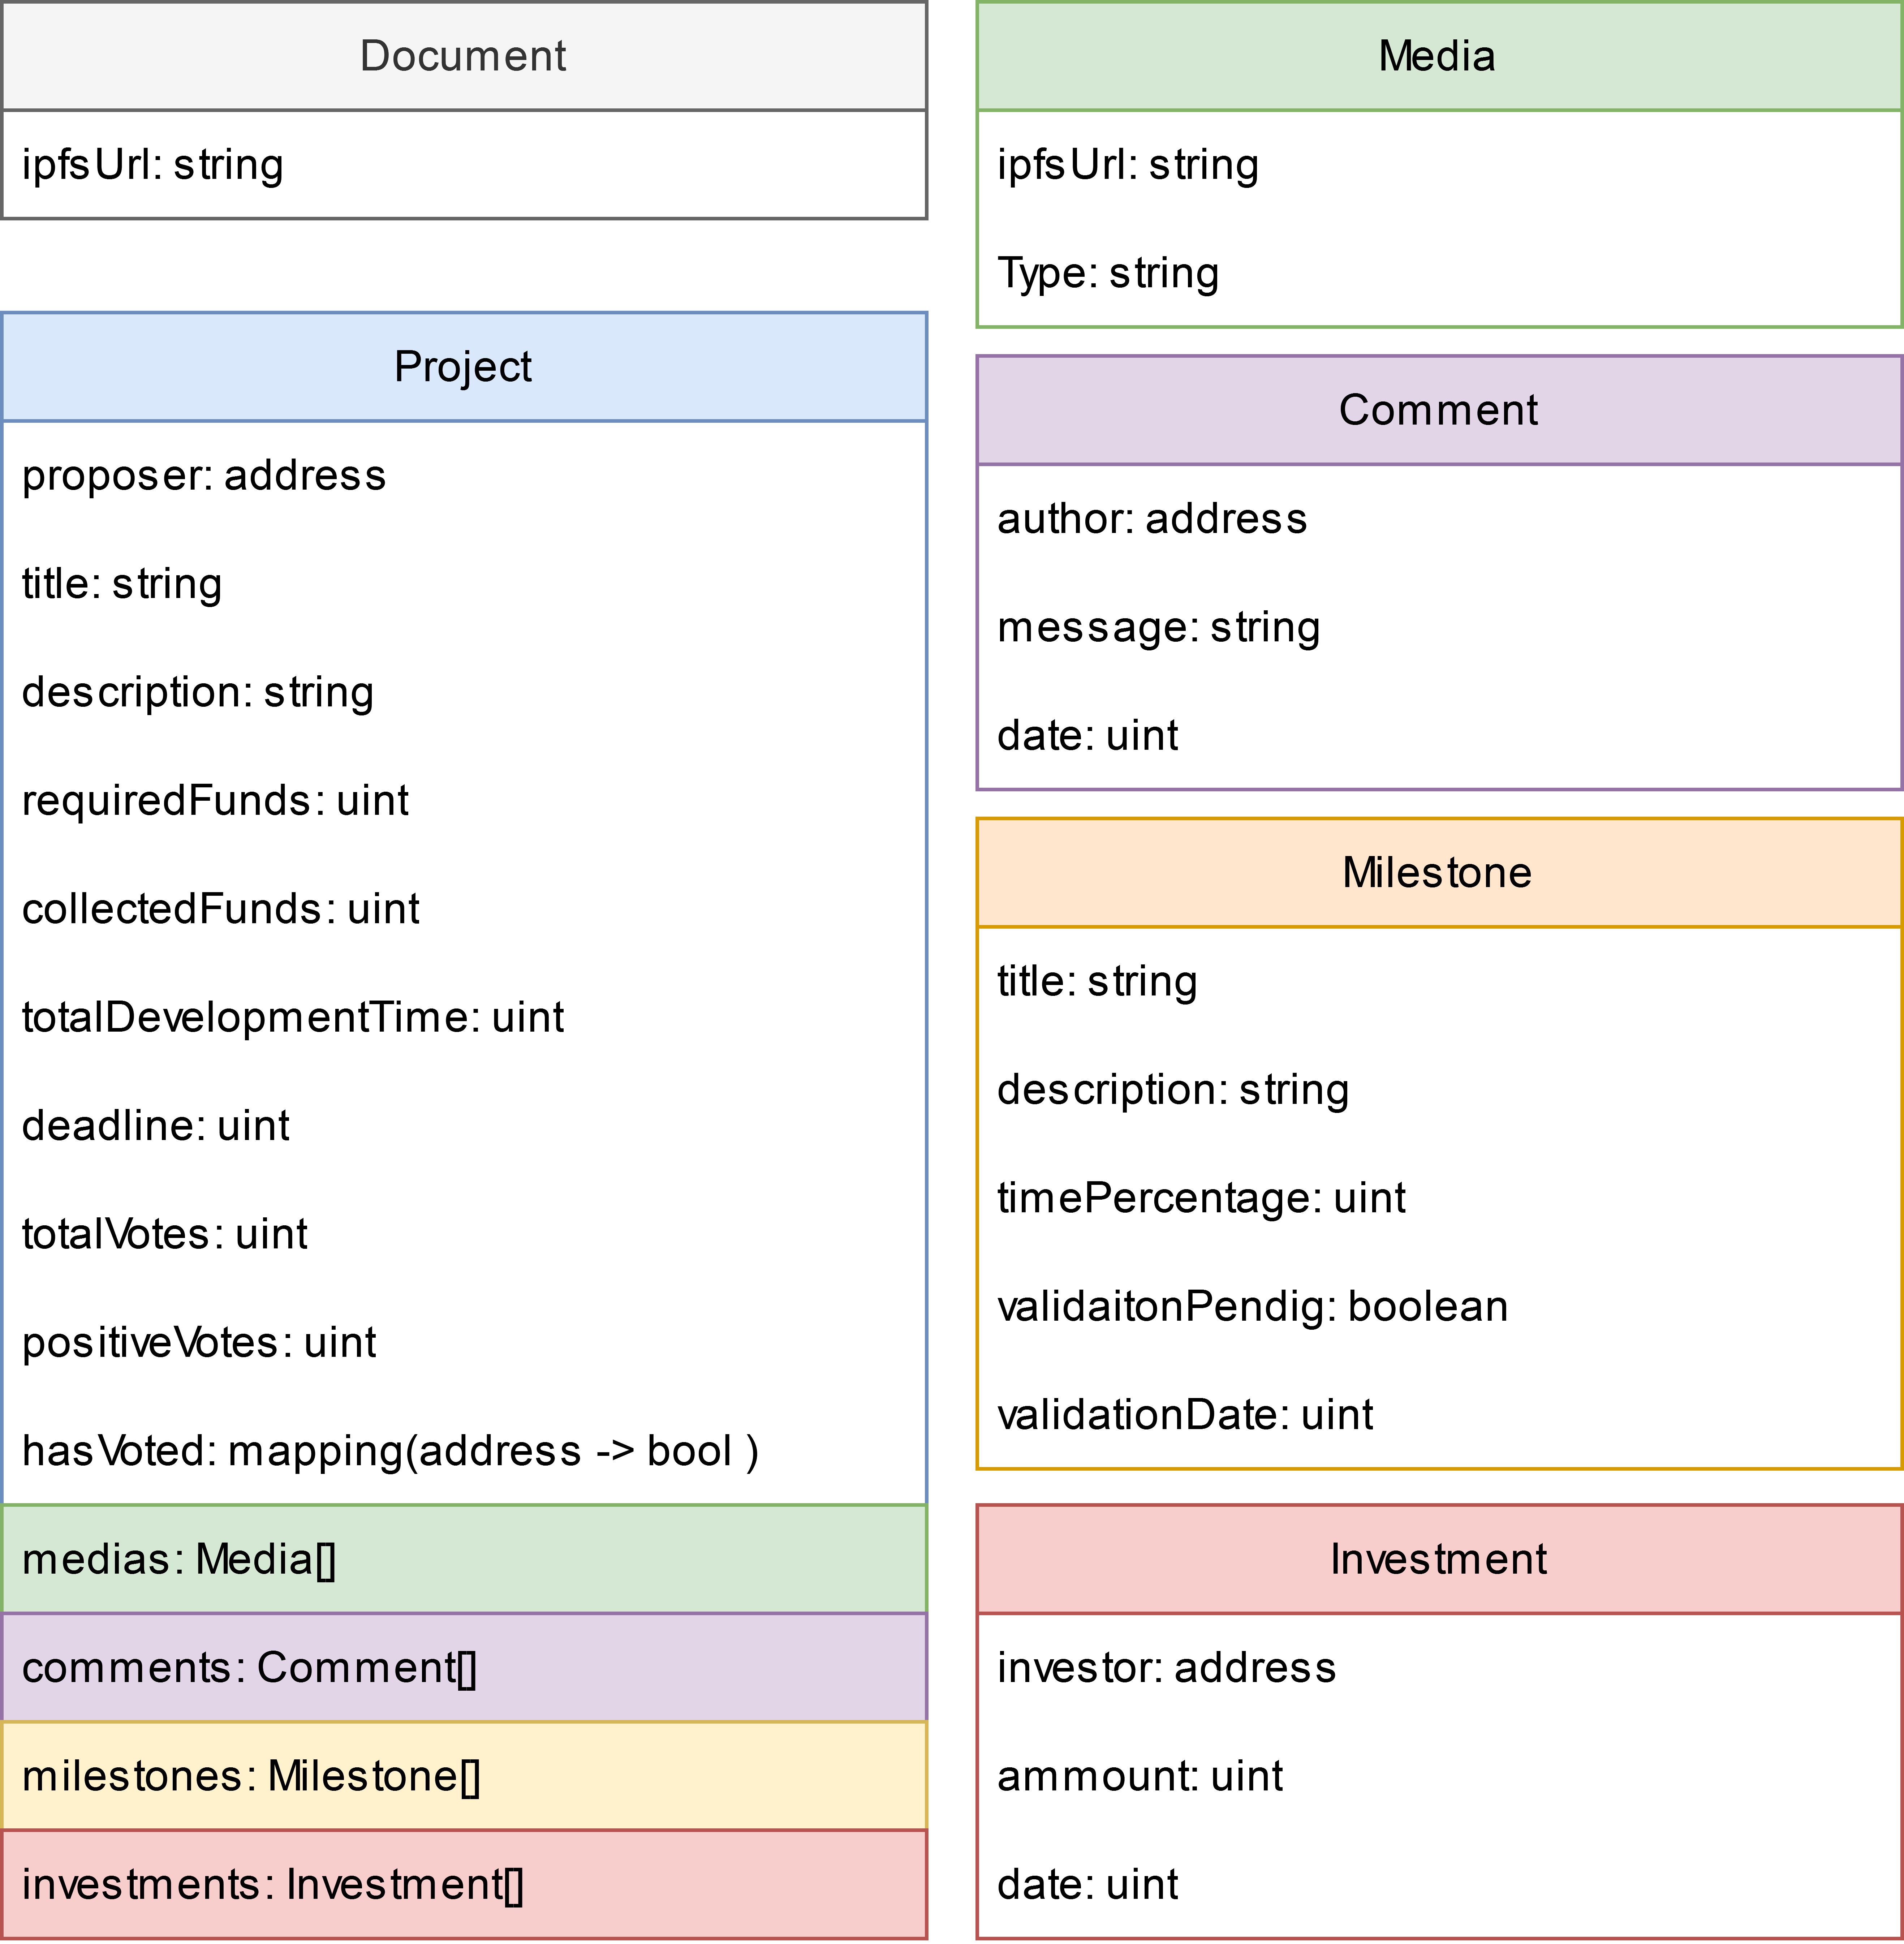
\includegraphics[width=1\textwidth]{img/diagramas/estructuras.png}
        \caption{Modelo - Estructura de los datos del smart contract.}
        \label{fig:configApi}
\end{figure}

\newpage

\paragraph{Project}

Esta estructura representa un proyecto y sus atributos, el smart contract poseerá un array de este tipo de datos, donde se almacenarán todos los datos necesarios.

\bigskip

La estructura alberga la dirección del proponente, el titulo, descripción del proyecto, además de los fondos requeridos en MATIC, los fondos obtenidos hasta el momento, el tiempo total necesario para su desarrollo, fecha limite para la siguiente fase, votos totales, votos totales positivos, mapping de quien ha votado.

\bigskip

Además, esta estructura poseerá un array de Media para almacenar fotos y videos, Comment para almacenar un historial de comentarios, Milestones para almacenar la lista de hitos y Investemtns para registrar un historial de quien ha invertido en el proyecto y cuanto.

\paragraph{Milestone}

La estructura de Milestone representa un Hito, este poseerá un titulo, descripción, porcentaje del tiempo necesario del total del proyecto para su realización, verificador si el hito está pendiente de validación, y fecha en formato UNIX cuando se ha validado.

\paragraph{Comment}

Esta estructura representa un comentario, y contiene la dirección del autor, el mensaje y la fecha en formato UNXI.

\paragraph{Investment}

Esta estructura contiene los datos necesarios para representar una inversión, siendo sus parámetros la dirección de la cuenta del inversor, la cantidad invertida y la fecha en formato UNIX.

\paragraph{Media}

Mediante esta estructura se representa un archivo multimedia subido a IPFS, la cual contiene el URL-HASH de IPFS del archivo subido y  el tipo ( foto / vídeo ).

\paragraph{Document}

Esta estructura representa un documento subido a IPFS, se usa principalmente para gestionar los certificados de los peritos, y contiene la URL-HASH de IFPS del modelo de datos de credenciales verificables de W3C\cite{w3c}.

\newpage

\subsubsection{Arquitectura del smart contract}

En este apartado se presenta una interfaz de los métodos y variables que se implementan en el smart contract de la prueba de concepto.

\bigskip

{\huge Variables y Structs}

\paragraph{ProjectState}
\textbf{Descripción:}
Enumeración para representar el estado de un proyecto.

\textbf{Valores del enumerador:}
\begin{itemize}
    \item PENDING: Estado pendiente de aprobación.
    \item FUNDING: Estado en proceso de financiamiento.
    \item FUNDED: Estado financiado completamente.
    \item CANCELLED: Estado cancelado.
\end{itemize}


\paragraph{Comment}
\textbf{Descripción:}
Estructura para representar un comentario en un proyecto.

\textbf{Atributos:}
\begin{itemize}
    \item \texttt{author}: Dirección del autor del comentario (address).
    \item \texttt{message}: Texto del comentario (string).
    \item \texttt{date}: Fecha del comentario (uint).
\end{itemize}

\paragraph{Investment}
\textbf{Descripción:}
Estructura para representar una inversión en un proyecto.

\textbf{Atributos:}
\begin{itemize}
    \item \texttt{investor}: Dirección del inversor (address).
    \item \texttt{amount}: Cantidad invertida (uint).
    \item \texttt{date}: Fecha de la inversión (uint).
\end{itemize}

\paragraph{Project}
\textbf{Descripción:}
Estructura para representar un proyecto en la plataforma.

\textbf{Atributos:}
\begin{itemize}
    \item \texttt{proposer}: Dirección del proponente del proyecto (address).
    \item \texttt{title}: Título del proyecto (string).
    \item \texttt{description}: Descripción del proyecto (string).
    \item \texttt{requiredFunds}: Fondos necesarios para el proyecto en Ether (uint).
    \item \texttt{collectedFunds}: Fondos recaudados en Ether (uint).
    \item \texttt{totalDevelopmentTime}: Tiempo total de desarrollo del proyecto en días (uint).
    \item \texttt{deadline}: Fecha límite para la siguiente fase (votación, financiación o validación de hitos) (uint).
    \item \texttt{totalVotes}: Total votos recibidos (uint).
    \item \texttt{positiveVotes}: Total votos positivos recibidos (uint).
    \item \texttt{state}: Estado del proyecto (ProjectState).
    \item \texttt{investments}: Array para controlar las inversiones de cada dirección en el proyecto (Investment[]).
    \item \texttt{comments}: Array para almacenar los comentarios del proyecto (Comment[]).
    \item \texttt{hasVoted}: Mapping para controlar quién ha votado el proyecto (mapping(address => bool)).
\end{itemize}

\newpage

{\huge Interfaz de las Funciones}

\paragraph{getProjectsCount}
\noindent
\textbf{Descripción:}
Devuelve el total de proyectos actuales en el smart contract.\\
\textbf{Parámetros:}
No tiene parámetros. \\
\textbf{Retorno:}
Devuelve un uint256 que representa el número total de proyectos.

\paragraph{proposeProject}
\noindent
\textbf{Descripción:}
Propone un nuevo proyecto para ser aprobado por la comunidad. \\
\textbf{Parámetros:}
\begin{itemize}
    \item \texttt{\_title}: Título del proyecto (string memory).
    \item \texttt{\_description}: Descripción del proyecto (string memory).
    \item \texttt{\_fundingGoal}: Cantidad de fondos (en Ether) necesarios para su formalización (uint).
    \item \texttt{\_totalDevelopmentTime}: Tiempo total (días) para su desarrollo (uint).
\end{itemize}
\textbf{Retorno:}
Devuelve el ID del proyecto (uint256).

\paragraph{getProject}
\noindent
\textbf{Descripción:}
Devuelve un proyecto dado un ID. \\
\textbf{Parámetros:}
\begin{itemize}
    \item \texttt{\_projectId}: ID del proyecto.
\end{itemize}
\textbf{Retorno:}
Devuelve una objeto con los siguientes elementos del proyecto:
\begin{itemize}
    \item \texttt{proposer}: Dirección del proponente (address memory).
    \item \texttt{title}: Título del proyecto (string memory).
    \item \texttt{description}: Descripción del proyecto (string memory).
    \item \texttt{requiredFunds}: Cantidad de fondos (en Ether) necesarios para su formalización (uint).
    \item \texttt{collectedFunds}: Cantidad de fondos (en Ether) recaudados hasta el momento (uint).
    \item \texttt{totalDevelopmentTime}: Tiempo total (días) para su desarrollo (uint).
    \item \texttt{deadline}: Días restantes hasta la siguiente fase, dependiendo del estado (uint).
    \item \texttt{status}: Estado actual del proyecto (enumerado: PEDING FUNDING, FUNDED, CANCELLED).
    \item \texttt{totalVotes}: Contador de la cantidad de votos totales (uint).
    \item \texttt{positiveVotes}: Contador de la cantidad de votos positivos del total (uint).
    \item \texttt{userVoted}: Booleano que indica si el usuario que solicita los datos ha votado en dicho proyecto (bool).
\end{itemize}


\paragraph{getCommentsCount}
\noindent
\textbf{Descripción:}
Devuelve la cantidad de comentarios de un proyecto dado un ID. \\
\textbf{Parámetros:}
\begin{itemize}
    \item \texttt{\_projectId}: ID del proyecto (uint).
\end{itemize}
\textbf{Retorno:}
Devuelve un entero que representa la cantidad de comentarios (uint).


\paragraph{addComment}
\noindent
\textbf{Descripción:}
Añade un comentario a un proyecto. \\
\textbf{Parámetros:}
\begin{itemize}
    \item \texttt{\_projectId}: ID del proyecto (uint).
    \item \texttt{\_comment}: comentario a añadir (string memory).
\end{itemize}
\textbf{Retorno:}
No devuelve ningún valor.

\paragraph{getComment}
\noindent
\textbf{Descripción:}
Devuelve un comentario dado un ID de proyecto y un ID de comentario. \\
\textbf{Parámetros:}
\begin{itemize}
    \item \texttt{\_projectId}: ID del proyecto (uint).
    \item \texttt{\_commentId}: ID del comentario (uint).
\end{itemize}
\textbf{Retorno:}
\begin{itemize}
    \item \texttt{author}: Address del autor del comentario (address).
    \item \texttt{message}: Contenido del comentario (string memory).
    \item \texttt{date}: Fecha en formato UNIX de cuando se añadió el comentario (uint).
\end{itemize}


\paragraph{getComments}
\noindent
\textbf{Descripción:}
Devuelve todos los comentarios de un proyecto. \\
\textbf{Parámetros:}
\begin{itemize}
    \item \texttt{\_projectId}: ID del proyecto (uint).
\end{itemize}
\textbf{Retorno:}
\begin{itemize}
    \item \texttt{comments}: Array de Comment (Comment[]).
\end{itemize}


\paragraph{voteProject}
\noindent
\textbf{Descripción:}
Permite a los miembros de la comunidad votar un proyecto propuesto. \\
\textbf{Parámetros:}
\begin{itemize}
    \item \texttt{\_projectId}: ID del proyecto (uint256).
    \item \texttt{\_positiveVote}: Voto a favor o en contra del proyecto (bool).
\end{itemize}
\textbf{Retorno:}
No devuelve ningún valor.


\paragraph{hasVoted}
\noindent
\textbf{Descripción:}
Devuelve si el usuario ha votado un proyecto. \\
\textbf{Parámetros:}
\begin{itemize}
    \item \texttt{\_projectId}: ID del proyecto (uint).
    \item \texttt{\_user}: Address de un usuario (address).
\end{itemize}
\textbf{Retorno:}
\begin{itemize}
    \item \texttt{bool}: Booleano que indica si el usuario ha votado o no en el proyecto (bool).
\end{itemize}


\paragraph{checkProjectApproval}
\noindent
\textbf{Descripción:}
Comprueba si un proyecto ha sido aprobado por la comunidad, en caso positivo se cambia el estado del proyecto. \\
\textbf{Parámetros:}
\begin{itemize}
    \item \texttt{\_projectId}: ID del proyecto (uint).
\end{itemize}
\textbf{Retorno:}
No devuelve ningún valor.


\paragraph{investInProject}
\noindent
\textbf{Descripción:}
Permite a los miembros de la comunidad financiar un proyecto aprobado. La cantidad invertida se obtienen desde los metadatos de la transacción. \\
\textbf{Parámetros:}
\begin{itemize}
\item \texttt{\_projectId}: ID del proyecto (uint256).
\end{itemize}
\textbf{Retorno:}
No devuelve ningún valor.


\paragraph{checkProjectFunding}
\noindent
\textbf{Descripción:}
Comprueba si un proyecto ha sido financiado, en caso de ser así, cambia el estado de dicho proyecto y transfiere lo recaudado al proponente. \\
\textbf{Parámetros:}
\begin{itemize}
\item \texttt{\_projectId}: ID del proyecto (uint256).
\end{itemize}
\textbf{Retorno:}
No devuelve ningún valor.


\paragraph{withdrawInvestment}
\noindent
\textbf{Descripción:}
Permite a los inversores retirar sus fondos si el proyecto se ha cancelado. \\
\textbf{Parámetros:}
\begin{itemize}
\item \texttt{\_projectId}: ID del proyecto (uint256).
\end{itemize}
\textbf{Retorno:}
No devuelve ningún valor.

\newpage
